\chapter{A Benchmark-Based Evaluation of Search-BasedCrash Reproduction}
\blfootnote{This chapter is published as a paper with two first authors. The author of this thesis and the other first author contributed equally to this work.}


\label{sec:jcrashpack:introduction}

Software crashes commonly occur in operating environments and are reported to developers for inspection.
When debugging, reproducing a reported crash is among the tasks a developer needs to do in order to identify the conditions under which the reported crash is triggered \cite{Zeller2009}.
To help developers in this process, various automated techniques have been suggested.
These techniques typically either use program \emph{runtime data} \cite{Artzi2008, Clause2007, Narayanasamy2005, Steven2000, Gomez2016, Bell2013, Cao2014, Rossler2013} or crash \emph{stack traces} \cite{BPT17concrash, soltani2017, Nayrolles2017, Xuan2015, Chen2015} to generate a test case that triggers the reported crash.  

When available, runtime data offer more information to accurately reproduce a crash. However, it also raises various concerns (for instance, privacy violation) and may induce a significant overhead during data collection \cite{Chen2015, Nayrolles2017, Rossler2013}. Instead, we focus on crash reproduction based on a crash stack trace generated by a failing system. Practically, those stack traces are collected from the logs produced by the operating environment or reported by users in an issue tracking system. Various auromated crash stack trace-based reproduction approaches have been implemented and evaluated on different benchmarks \cite{soltani2017, Nayrolles2017, Xuan2015, Chen2015}. However, those benchmarks contains a limited number of crashes and associated stack traces.

In a recent study, we presented a search-based approach called \evocrash, which applies a guided genetic algorithm to search for a crash reproducing test case \cite{soltani2017}, and demonstrated its relevance for debugging \cite{Soltani2018a}.
We conducted an empirical evaluation on 54 crashes from commonly used utility libraries to compare \evocrash with state-of-the-art techniques for crash reproduction \cite{soltani2017}.
This was enough to show that the search-based crash reproduction outperformed other approaches based on backward symbolic execution \cite{Chen2015}, test case mutation \cite{Xuan2015}, and model-checking \cite{Nayrolles2017}, evaluated on smaller benchmarks.

However, all those crashes benchmarks were not selected to reflect challenges that are likely to occur in real life stack traces, raising threats to external validity.
Thus the questions whether the selected applications and crashes were sufficiently representative, if \evocrash will work in other contexts, and what limitations are still there to address, remained unanswered.

The goal of this chapter is to facilitate sound empirical evaluation on automated crash reproduction approaches.
To that end, we devise a new benchmark of real-world crashes, called \crashpack.
It contains 200 crashes from seven actively maintained open-source and industrial projects.
These projects vary in their domain application and include an enterprise wiki application, a distributed RESTful search engine, several popular APIs, and a mocking framework for unit testing Java programs. 
\crashpack is extensible, and can be used for large-scale evaluation and comparison of automated crash reproduction techniques for Java programs.

To illustrate the use of \crashpack, we adopt it to extend the reported evaluation on \evocrash~\cite{soltani2017} and identify the areas where the approach can be improved.
In this experience report, we provide an account of the cases that were successfully reproduced by \evocrash (87 crashes out of 200). 
We also analyze all failed reproductions and distill 14 categories of research and engineering limitations that negatively affected reproducing crashes in our study. 
Some of those limitations are in line with challenges commonly reported for search-based structural software testing in the community \cite{xiao2011precise, McMinn2011, Fraser2014b} and others are specific to search-based crash reproduction.

Our categorization of challenges indicates that environmental dependencies, code complexity, and limitations of automated input data generation often hinder successful crash reproduction.
In addition, stack frames (i.e., lines in a stack trace), pointing to varying types of program elements, such as interfaces, abstract classes, and anonymous objects, influence the extent to which a stack trace-based approach to crash reproduction is effective.

Finally, we observe that the percentage of successfully reproduced crashes drops from 85\% (46 crashes out of 54 reported by Soltani \etal \cite{Soltani2018a}) to 43\% (87 out of 200) when evaluating crashes that are from industrial projects. 
In our observations, generating input data for microservices, and unit testing for classes with environmental dependencies, which may frequently exist in enterprise applications, are among the major reasons for the observed drop in the reproduction rate.
These results are consistent with the paradigm shift to context-based software engineering research that has been proposed by Briand et al. \cite{Briand2017a}.

The key contributions of this chapter are:
\begin{itemize}
\item \crashpack,\footnote{Available at \url{https://github.com/STAMP-project/JCrashPack}.} a carefully composed benchmark of 200 crashes, as well as their correct system version and its libraries, from seven real-world Java projects, together with an account of our manual analysis on the characteristics of the selected crashes and their constituting frames, including size of the stack traces, complexity measures, and identification of buggy and fixed versions.

\item \exrunner,\footnote{Available at \url{https://github.com/STAMP-project/ExRunner}} a Python library for automatically running experiments with crash reproduction tools in Java.

\item Empirical evidence,\footnote{A replication package for \evocrash results, their automated analysis, and the results of our manual analysis is available at \url{https://github.com/STAMP-project/EvoCrash-JCrashPack-application}.} demonstrating the effectiveness of search-based crash reproduction on real world crashes taken from \crashpack.

\item The identification of 14 categories of research and engineering challenges for search-based crash reproduction that need to be addressed in order to facilitate uptake in practice of crash reproduction research.

\end{itemize}
%\todoall{Please review the item for \exrunner!}

The remainder of the chapter is structured as follows:
Sections~\ref{sec:jcrashpack:benchmarkdesign} to \ref{sec:jcrashpack:ExRunner} describe the design protocol for the benchmark, the resulting benchmark \crashpack, as well as the \exrunner tool to run experiments on \crashpack.
Sections~\ref{sec:jcrashpack:evocrashevalsetup} to \ref{sec:jcrashpack:challenges} cover the experimental setup for the \evocrash evaluation, the results from our evaluation, and the results challenges that we identified through our evaluation.
Sections~\ref{sec:jcrashpack:discussion} to \ref{sec:jcrashpack:conclusion} provide a discussion of our results and future research directions, an analysis of the threats to validity, and a summary of our overall conclusions.





% \section{Background and related work}
% \label{sec:jcrashpack:background}
% 
\subsection{Automated Crash Reproduction}
Software crashes commonly occur in operating environments and are reported to developers for inspection.
When debugging, reproducing a reported crash is among the tasks a developer needs to do in order to identify the conditions under which the reported crash is triggered \cite{Zeller2009, BellerICSE2018}.
In particular, for Java programs, when a crash occurs, an exception is thrown. A developer strives to reproduce it to understand its cause, then fix the bug, and finally add a (non-)regression test to avoid reintroducing the bug in future versions. 

Manual crash reproduction can be a challenging and labor-intensive task for developers: it is often an iterative process that requires setting the debugging environment in a similar enough state as the environment in which the crash occurred~\cite{Zeller2009}.

To help developers in this process, various automated techniques have been suggested.
These techniques can be divided into three categories, based on the kind of data used for crash reproduction: \emph{record-replay approaches}~\cite{Artzi2008, Clause2007, Narayanasamy2005, Steven2000, Gomez2016, Bell2013, Cao2014} record data from the running program; \emph{post-failure approaches}~\cite{Rossler2013, YZW17descry,Weeratunge2010, Leitner2007, Leitner2009, Kifetew2013, Kifetew2014} collect data from the crash, like a memory dump; and \emph{stack-trace based post-failure}~\cite{BPT17concrash,soltani2017,Nayrolles2017,Xuan2015,Chen2015} use only the stack trace produced by the crash. We briefly describe each category hereafter.

\paragraph{Record-replay approaches.}

These approaches record the program runtime data and use them during crash reproduction. The main limitation is the availability of the required data. Monitoring software execution may violate privacy by collecting sensitive data, the monitoring process can be an expensive task for the large scale software, and may induce a significant overhead \cite{Chen2015, Nayrolles2017, Rossler2013}.
%
Tools like \textrm{ReCrash} \cite{Artzi2008}, \textrm{ADDA} \cite{Clause2007}, \textrm{Bugnet} \cite{Narayanasamy2005}, \textrm{jRapture} \cite{Steven2000}, \textrm{MoTiF} \cite{Gomez2016}, \textrm{Chronicler} \cite{Bell2013}, and \textrm{SymCrash} \cite{Cao2014} fall in this category.


\paragraph{Post-failure approaches.}

Techniques from this category use the software data collected directly after the occurrence of a failure. For instance, \textrm{RECORE} \cite{Rossler2013} applies a search-based approach to reproduce a crash by using the stack trace and a core dump, produced by the system when the crash happened, to guide the search.
% Instead, \evocrash only considers the stack trace (usually provided when a bug is reported in an issue tracker) and a distance, similar to the one described by Rossler \etal \cite{Rossler2013}, to guide the search.

Although these tools limit the quantity of monitored and recorded data, the availability of such data still represents a challenge. 
Yu \etal \cite{YZW17descry} addressed this issue for system-level concurrency failure reproduction by introducing \textrm{DESCRY}. 
This approach only uses the default execution logs and applies both static and dynamic analysis combined with symbolic execution to generate the input data and interleaving schedule. 
However, even this approach suffers from two limitations: 
\begin{inparaenum}[(i)]
\item since this tool relies on symbolic execution, applying it on the large and complex projects leads to path explosion;
\item the performance of this tool is strongly linked to the quality of the software log.
\end{inparaenum}
%
Other \textit{post-failure approaches} inlcude: Weeratunge \etal \cite{Weeratunge2010}, Leitner \etal \cite{Leitner2007, Leitner2009}, and Kifetew \etal \cite{Kifetew2013, Kifetew2014}.

\paragraph{Stack-trace based post-failure.}

Recent studies in crash reproduction \cite{BPT17concrash,soltani2017,Nayrolles2017,Xuan2015,Chen2015} focuses on utilizing data only from a given crash stack trace to enhance the practical application. 
%
Table~\ref{tab:ant49755} illustrates an example of a crash stack trace from Apache Ant\footnote{ANT-49755: \url{https://bz.apache.org/bugzilla/show_bug.cgi?id=49755} } ~\cite{ant} which is comprised of a crash type (\texttt{java.lang.Null\-Pointer\-Exception}) and a stack of frames pointing to all method calls that were involved in the execution when the crash happened.
From a crash stack frame, we can retrieve information about: the crashing method, the line number in the method where the crash happened, and the fully qualifying name of the class where the crashing method is declared.

\begin{table*}[t]
\centering
\caption{The crash stack trace for Apache Ant-49755.}
\label{tab:ant49755}
\begin{tabular}{c|l}
\multicolumn{2}{l}{java.lang.\textbf{NullPointerException}:}\\
\hline
\textbf{Level} & \textbf{Frame} \\
\hline
1 & \textbf{at} org.apache.tools.ant.util.FileUtils.\textbf{createTempFile}(FileUtils.java:\textbf{888})\\
2 & \textbf{at} org.apache.tools.ant.taskdefs.TempFile.\textbf{execute}(TempFile.java:\textbf{158})\\
3 & \textbf{at} org.apache.tools.ant.UnknownElement.\textbf{execute}(UnknownElement.java:\textbf{291}) \\
\end{tabular}
\end{table*}

The state of the research in crash reproduction \cite{Zamfir2010, jin2012bugredux, BPT17concrash, soltani2017, Nayrolles2017, Xuan2015, Chen2015} aims at generating test code that, once executed, produces a stack trace that is as similar to the original one as possible. They, however, differ in their means to achieve this task. 

\textrm{ESD} \cite{Zamfir2010}, a debugger based on execution synthesis, uses forward symbolic execution and static analysis to reach reproduction. This tool focuses more on concurrency and memory safety bugs.
Similarly, \textrm{BugRedux} \cite{jin2012bugredux} uses forward symbolic execution. \textrm{BugRedux} is a crash reproduction tool for C programs.

Since these two tools rely on forward symbolic execution, they can be applied only on medium-size applications. Also, as illustrated by Braione \etal \cite{braione2017tardis}, symbolic execution test generation approaches face limitations when generating complex input data structures.
To address these limitations, \textrm{STAR} \cite{Chen2015} applies optimized backward symbolic execution and uses a novel technique for method sequence composition to generate a unit test that satisfies the computed preconditions, and eventually reproduces the target crash. 
However, as reported by Chen \etal \cite{Chen2015}, \textrm{STAR} still suffers from the path explosion problem stemming from utilizing symbolic execution. 
It only supports 3 types of exceptions: explicitly thrown exceptions, \texttt{NullPointerException}, and \texttt{ArrayIndexOutOfBoundsException}.  

\textrm{JCHARMING} \cite{Nayrolles2017} applies model checking to reproduce the reported bugs. To prevent state explosion in the model, it utilizes program slicing.
Since \textrm{JCHARMING} can be applied to any frame from a given crash stack trace, the approach can reproduce any fraction of the target crash stack trace. 

\textrm{MuCrash} \cite{Xuan2015} is based on exploiting existing test cases written by developers and mutating them until they trigger the target crash.
Test case mutation in \textrm{MuCrash} is directed by selecting tests for the classes included in the target crash stack trace. 

Finally, \textrm{Concrash} \cite{BPT17concrash} focuses on reproducing \textit{concurrency} failures that violate thread-safety of a class.
\textrm{Concrash} iteratively generates test code and looks for a thread interleaving that triggers a concurrency crash.
In order to steer the test generation process and avoid expensive computations, \textrm{Concrash} applies the pruning strategies to avoid redundant and irrelevant test code. In contrast to other crash reproduction techniques, \textrm{Concrash} only reproduces the minority of the crashes in the issue tracking systems. As reported by Yuan \etal \cite{Yuan2014}, inter-leaving crashes cause only 10\% of failures in the distributed data-intensive systems. Besides, Coelho \etal \cite{Coelho2015} state that this number is even lower in Android applications (2.9\%).

\subsection{Search-based Crash Reproduction With \evocrash}

Search-based algorithms have been increasingly used for software engineering problems since they are shown to suite complex, non-linear problems, with multiple optimization objectives that may conflict or competing~\cite{harman12trends}.
\evocrash \cite{soltani2017, Soltani2018a} is a search-based approach to crash reproduction, which applies a \textit{guided genetic algorithm} to search for a unit test that reproduces the target crash. They have shown that this search-based technique outperforms other automated crash reproduction approaches.

\evocrash takes as input a stack trace with one of its frames set as the \emph{target frame}. 
The target frame is composed of a
(i) \emph{target class}, the class to which the exception has been propagated; a
(ii) \texttt{target method}, the method in that class; and a
(iii) \emph{target line}, the line in that method where the exception has been propagated. 
It then seeks to generate a unit test that replicates the given stack trace from the target frame (at level $n$) to the deepest frame (at level 1). 
For instance, if we pass the stack trace in Table \ref{tab:ant49755} as the given trace and indicate the second frame as the target frame (level 2), the output of \evocrash will be a unit test for the class \texttt{TempFile} which replicates the first two frames of the given stack trace with the same type of the exception (\texttt{NullPointerException}).

\subsubsection{Guided genetic algorithm}
\label{sec:background:evocrash:guidedalg}
The search process in \evocrash begins by randomly generating unit tests for the target frame.
In this phase, called \emph{guided initialization}, the target method corresponding to the selected frame (i.e., the \emph{failing method} to which the exception is propagated) is injected in every randomly generated unit test.
During subsequent phases of the search, \emph{guided crossover} and \emph{guided mutation}, standard evolutionary operations are applied to the unit tests.
However, applying these operations involves the risk of losing the injected failing method.
Therefore, the algorithm ensures that only unit tests with the injected failing method call remain in the evolution loop. 
If the generated test by crossover does not contain the failing method, the algorithm replaces it with one of its parents. 
Also, if the resulting test does not contain the failing method after a mutation, the algorithm redoes the mutation until the failing method is added to the test again.
The search process continues until either the search budget is over or a crash reproducing test case is found.

To evaluate the generated tests, \evocrash applies the following weighted sum fitness function \cite{Soltani2018a} (called \CrashFunction, hereafter) to a generated test $t$:
%
\rowcolors{1}{}{}
\begin{equation} \label{eq:fitnessfunction}
f(t) = 
\left\{
  \begin{array}{lcr}
    3 \times d_{s}(t) + 2 \times max(d_{except}) + max(d_{trace})   && \textit{if the line is not reached}\\
    3 \times min(d_{s}) + 2 \times d_{except}(t) + max(d_{trace})   && \textit{if the line is reached}\\
    3 \times min(d_{s}) + 2 \times min(d_{except}) + d_{trace}(t)   && \textit{if the exception is thrown}
  \end{array}
\right.
\end{equation}
\rowcolors{1}{}{gray!15}
%
Where:
%
\begin{itemize}
\item $d_{s} \in [0,1]$ indicates the distance between the execution of $t$ and the target statement $s$ located at the target line. 
This distance is computed using the \textit{approach level}, measuring the minimum number of control dependencies between the path of the code executed by $t$ and $s$, and normalized \textit{branch distance}, scoring how close $t$ is to satisfying the branch condition for the branch on which$s$ is directly control dependent \cite{McMinn2004}. 
If the target line is reached by the test case, $d_{l}(t)$ equals to $0.0$;
%
\item $d_{except}(t) \in \{0,1\}$ indicates if the target exception is thrown ($d_{e} = 0$) or not ($d_{e} = 1$);
%
\item $d_{trace}(t) \in [0,1]$ indicates the similarity of the input stack trace and the one generated by $t$ by looking at class names, methods names and line numbers;
%
\item $max(\cdot)$ denotes the maximum possible value for the function.
\end{itemize}
%
Since the stack trace similarity is relevant only if the expected exception is thrown by $t$, and the check whether the expected exception is thrown or not is relevant only if the target line where the exception propagates is reached, $d_{except}$ and $d_{trace}$) are computed only upon the satisfaction of two \emph{constraints}: the target exception has to be thrown in the target line $s$ and the stack trace similarity should be computed only if the target exception is actually thrown. 

Unlike other stack trace similarity measures (e.g., \cite{Rossler2013}), Soltani \etal \cite{Soltani2018a} do not require two stack traces to share the same common prefix to avoid rejecting stack traces where the difference is only in one intermediate frame. Instead, for each frame, $d_{trace}(t)$ looks at the closest frame and computes a distance value. Formally, for an original stack trace $S^*$ and a test case $t$ producing a stack trace $S$, $d_{trace}(t)$ is defined as follows:
%
\rowcolors{1}{}{}
\begin{equation}
d_{trace}(t) = \varphi \left( \sum_{f^* \in S^*} min \left\lbrace \mathit{diff}(f^*, f) : f \in S \right\rbrace \right)
\end{equation}
\rowcolors{1}{}{gray!15}
%
Where $\varphi (x) = x / (x+1)$ is a normalization function \cite{McMinn2004} and \textit{diff}$(f^*, f)$ measures the difference between two frames as follows: 
%
\rowcolors{1}{}{}
\begin{equation}
\mathit{diff}(f^{**}, f) = 
\left\{
  \begin{array}{lcr}
    3 && \textit{if the classes are different}\\
    2  && \textit{if the classes are equal but the methods are different}\\
     \varphi \left( \vert l^* - l \vert \right)   && \textit{otherwise}
  \end{array}
\right.
\end{equation}
\rowcolors{1}{}{gray!15}
%
Where $l$ (resp. $l^*$) is the line number of the frame $f$ (resp. $f^*$).

Each of the three components if the fitness function defined in Equation \ref{eq:fitnessfunction} ranges from $0.0$ to $1.0$, the overall fitness value for a given test case ranges from $0.0$ (crash is fully reproduced) to $6.0$ (no test was generated), depending on the conditions it satisfies. 


\begin{table*}[t]
	\centering
	\caption{The number of crashes used in each crash reproduction tool experiment, the gained reproduction by them, and the involved projects.}
	\label{tab:background:represults}
	\small
\begin{tabular}{ l | c c c } 
\textbf{Tool} & \textbf{Reproduced/Total} & \textbf{Rate} & \textbf{Projects} \\
\hline 
\textbf{ EvoCrash~\cite{soltani2017, Soltani2018a}} & 46/54 & 85\% & \begin{tabular}[x]{@{}c@{}}Apache Commons Collections\\Apache Ant \\Apache
Log4j \\ActiveMQ \\DnsJava \\ JFreeChart \end{tabular} \\
%
\textbf{ EvoSuite~\cite{Soltani2018a}}  & 18/54 & 33\% & 
\begin{tabular}[x]{@{}c@{}}Apache Commons Collections\\Apache Ant \\Apache
Log4j \\ActiveMQ \\DnsJava \\ JFreeChart \end{tabular} \\
%
\textbf{ STAR~\cite{Chen2015}} & 30/51 & 59\% &
\begin{tabular}[x]{@{}c@{}}Apache Commons Collections\\Apache Ant \\Apache
Log4j \end{tabular} \\
%
\textbf{ MuCrash~\cite{Xuan2015}} & 8/12 & 66\%  &
\begin{tabular}[x]{@{}c@{}}Apache Commons Collections \end{tabular}\\
%
\textbf{ JCharming\cite{Nayrolles2017}} & 8/12 & 66\% &
\begin{tabular}[x]{@{}c@{}}Apache Ant \\Apache
Log4j \\ActiveMQ \\DnsJava \\ JFreeChart \end{tabular} \\
\end{tabular}
\end{table*}

\subsubsection{Comparison with the state-of-the-art}


\paragraph{Crash reproduction tools.}
%
Table \ref{tab:background:represults} presents the number of crashes used in the benchmarks used to evaluated stack-trace based post-failure crash reproduction tools as well as their crash reproduction rates. 
\evocrash has been evaluated on various crashes reported in other studies and has the highest reproduction rate.

%Unfortunately, as explained by Soltani \etal \cite{soltani2017, Soltani2018a}, other crash reproduction tools are not publicly available, and the reported comparisons in these studies are performed based on results published in \cite{Chen2015, Nayrolles2017, Xuan2015}. 

\paragraph{\evosuite{}.}
%
Table \ref{tab:background:represults} also reports the comparison of \evocrash with \evosuite, using exception coverage as the primary objective, applied by Soltani \etal \cite{Soltani2018a}. All the crashes reproduced by \evosuite could also be reproduced by \evocrash on average 170\% faster and with a higher reproduction rate. 


\subsubsection{Usefulness for debugging}

When reproducing a stack trace with \evocrash, there is no guarantee that the generated test completely reproduces the conditions in which the crash happened in the first place. Besides the random nature of search-based approaches, test cases are generated at the unit level, while crashes usually happen at the system level. However, rather than reproducing the exact same conditions of the crash, the goal of crash reproduction is to help developers fix the underlying bug.

Chen \etal \cite{Chen2015} introduced a usefulness criterion for the crash reproduction approaches. 
According to this criterion, a crash reproducing test is useful to the developers if it covers the buggy frame, \ie if the target frame for which the reproduction is successful is higher than the frame that points to the buggy method.
Soltani \etal \cite{Soltani2018a} refined that criterion through a controlled experiment with 35 master students in computer science and two crashes to assess the degree to which the tests generated by \evocrash helps to debug code. 
Their results indicate that the reproducing tests generated by \evocrash help the participants to fix the bugs more often, although not significantly, and significantly faster. 
They confirmed the usefulness criterion defined by the Chen \etal \cite{Chen2015}, but also found evidence that test cases categorized as not useful, according to this criterion, can still help developers fix the bug.




\section{Benchmark Design}
\label{sec:jcrashpack:benchmarkdesign}

Benchmarking is a common practice to assess a new technique and compare it to the state of the art \cite{Sim2003}.
For instance, SF110 \cite{Fraser2014b} is a sample of 100 Java projects from SourceForge, and 10 popular Java projects from GitHub, that may be used to assess (search based) test case selection techniques.
In the same way, Defects4J \cite{just2014defects4j} is a collection of bugs coming from popular open-source projects: for each bug, a buggy and a fixed version of the projects, as well as bug revealing test case, are provided. Defects4J is aimed to assess various testing techniques like test case selection or fault localization.

In their previous work, Soltani et al. \cite{soltani2017}, Xuan et al. \cite{Xuan2015}, and Chen and Kim \cite{Chen2015} used Apache Commons Collections~\cite{commonscollections}, Apache Ant~\cite{ant}, and Apache Log4j~\cite{log4j} libraries.
In addition to  Apache Ant and Apache Log4j, Nayrolles et al. \cite{Nayrolles2017} used bug reports from 8 other open-source software.

In this chapter we enhance previous efforts to build a benchmark dedicated to crash reproduction by collecting cases coming from both state of the art literature and actively maintained industrial open-source projects with well documented bug trackers.

\subsection{Projects Selection Protocol}

As Table \ref{tab:background:represults} clearly shows, current crash reproduction tools are not evaluated using a common benchmark.
This hampers progress in the field as it makes it hard to compare approaches.
To be able to perform analysis of the results of a crash reproduction attempt, we define the following \emph{benchmark requirements} for our benchmark:
\begin{itemize}
\item[ \textbf{BR1},] to be part of the benchmark, the projects should have openly accessible binaries, source code, and crash stack traces (in an issue tracker for instance);
\item[ \textbf{BR2},] they should be under active maintenance to be representative of current software engineering practices and ease communication with developers;
\item[ \textbf{BR3},] each stack trace should indicate the version of the project that generated the stack trace; and
\item[ \textbf{BR4},] the benchmark should include projects of varying size.
\end{itemize}

To best of our knowledge, there is no benchmark fulfilling those requirements. The closest benchmark is Defects4j. However, only 25\% of the defects manifest through a crash stack trace (\textbf{BR1}) and the projects are relatively small (\textbf{BR4}). To address those limitations, we built a new benchmark dedicated to the crash reproduction tools.

%We have no restriction on the stack traces to consider, but want some diversity in the kinds of projects: APIs, web-applications, etc.
%We favor quality over quantity: a small set of projects with many stack traces representing different types of crashes, as the effort of manual analysis and setting up the test environment can be substantial.

To build our benchmark, we took the following approach.
First, we investigated projects collected in SF1\-10~\cite{Fraser2014b} and Defects4J~\cite{just2014defects4j} as state of the art benchmarks.
However, as most projects in SF110 have not been updated since 2010 or earlier, we discarded them from our analysis (\textbf{BR2}).
%
From Defects4J, we collected 73 cases where bugs correspond to actual crashes: i.e., the execution of the test case highlighting the bug in a given buggy version of a project generates a stack trace that is not a test case assertion failure. 

As also discussed by Fraser and Arcuri \cite{Fraser2014b}, to increase the representativeness of a benchmark, it is important to include projects that are popular and attractive to end-users.
Additionally to Defects4J, we selected two industrial open-source projects: XWiki~\cite{xwiki} and Elasticsearch \cite{elasticsearch}.
XWiki is a popular enterprise wiki management system.
Elasticsearch, a distributed RESTful search and analytic engine, is one of the ten most popular projects on GitHub\footnote{This selection was performed on 26/10/2017.}.
To identify the top ten popular projects from Github, we took the following approach:
%
\begin{inparaenum}[(i)]
\item we queried the top ten projects that had the highest number of forks;
\item we queried the top ten projects that had the highest number of stars;
\item we queried the top ten trending projects; and
\item took the intersection of the three.
\end{inparaenum}

Four projects were shared among the above top-ten projects, namely: Java-design-patterns~\cite{jdp}, Dubbo\cite{dubbo}, RxJava~\cite{rxjava}, and Elasticsearch.
To narrow down the scope of the study, we selected Elasticsearch, which ranked the highest among the four shared projects.


\subsection{Stack Trace Collection And Preprocessing}

For each project, we collected stack traces to be reproduced as well as the project binaries, with specific versions on which the exceptions happened.

\paragraph{Defects4J.}
%
From the 395 buggy versions of the Defects4J projects, we kept only the bugs relevant to our crash reproduction context (73 cases), i.e., the bugs that manifest as crashes. We manually inspected the stack traces generated by the failing tests and collected those which are not JUnit assertion failures (i.e., those which are due to an exception thrown by the code under test and not by the JUnit framework).
For instance, for one stack trace from the Joda-Time project:
%
\begin{lstlisting}[basicstyle=\scriptsize\ttfamily,breaklines=true,numbers=left,firstnumber=0]
java.lang.IllegalArgumentException:
  at org.joda.time.Partial.<init>(Partial.java:224)
  at org.joda.time.Partial.with(Partial.java:466)
  at org.joda.time.TestPartial_Basics.testWith_baseAndArgHaveNoRange(...)
\end{lstlisting}
%
We only consider the first and second frames (lines 1 and 2).
The third and following lines concern testing classes of the project, which are irrelevant for crash reproduction.
They are removed from the benchmark, resulting in the following stack trace with two frames:
%
\begin{lstlisting}[basicstyle=\scriptsize\ttfamily,breaklines=true,numbers=left,firstnumber=0]
java.lang.IllegalArgumentException:
  at org.joda.time.Partial.<init>(Partial.java:224)
  at org.joda.time.Partial.with(Partial.java:466)
\end{lstlisting}
%
We proceeded in the same way for each Defects4J project and collected a total of 73 stack traces coming from five (out of the six) projects: JFreeChart, Commons-lang, Commons-math, Mockito, and Joda-Time. All the stack traces generated by the Closure compiler test cases are JUnit assertion failures.

\paragraph{Elasticsearch.}
%
Crashes for Elasticsearch are publicly reported to the issue tracker of the project on GitHub\footnote{\url{https://github.com/elastic/elasticsearch/issues}}.
Therefore, we queried the reported crashes, which were labelled as bugs, using the following string \texttt{"exception is:issue label:bug"}.
From the resulting issues ($600$ approx.), we manually collected the most recent ones (reported since 2016), which addressed the following:
\begin{inparaenum}[(i)]
\item the version which crashed was reported,
\item the issue was discussed by the developers and approved as a valid crash to be fixed.
\end{inparaenum}
The above manual process resulted in 76 crash stack traces.

\paragraph{XWiki.}
%
XWiki is an open source project which has a public issue tracker\footnote{\url{https://jira.xwiki.org/browse/XWIKI/}}.
We investigated first 1000 issues which are reported for XWIK-7.2 (released in September 2015) to XWIK-9.6 (released in July 2017).
We selected the issues where:
\begin{inparaenum}[(i)]
\item the stack trace of the crash was included in the reported issue, and
\item the reported issue was approved by developers as a valid crash to be fixed.
\end{inparaenum}
Eventually, we selected a total of 51 crashes for XWIKI.



\section{The \crashpack Benchmark}
\label{sec:jcrashpack:benchmark}

The result of our selection protocol is a benchmark with 200 stack traces called \emph{\crashpack}. 
For each stack trace, based on the information from the issue tracker and the Defects4J data, we collected: the \emph{Java project} in which the crash happened, the \emph{version} of the project where the crash happened and (when available) the \emph{fixed version}  or the fixing commit reference of the project; the \emph{buggy frame} (i.e., the frame in the stack trace targeting the method where the bug lays); and the \emph{Cyclomatic Complexity Number (CCN)} and the \emph{Non-Com\-men\-ting Sources Statements (NCSS)} of the project, presented in Figure \ref{fig:ccnncssperapp}. 
Due to the manual effort involved in filtering, verifying and cleaning up stack traces, issues, the collection of stack traces and binaries (including the project's dependencies binaries) took about 4.5 person-months in total.

\begin{figure}[t]
  \centering
  \subfloat[Average methods Cyclomatic Complexity Number (CCN)]{%
  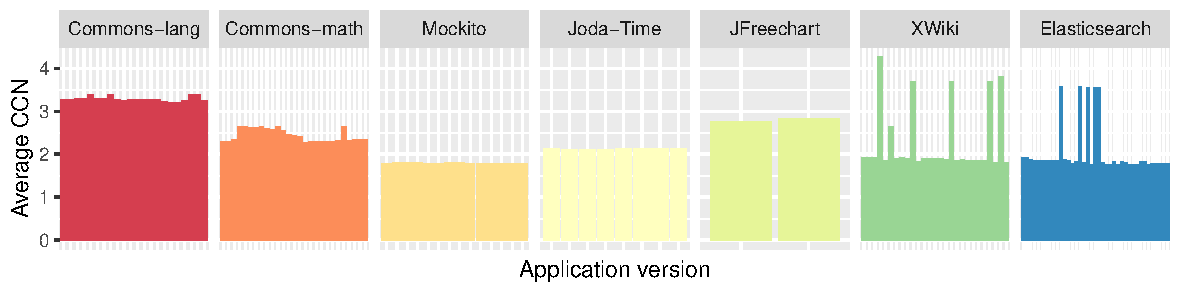
\includegraphics[width=0.98\textwidth]{papers/jcrashpack/benchmark-ccn-per-app-histogram}
  \label{fig:ccnperapp}
  }
  \subfloat[Thousands of Non-Com\-men\-ting Sources Statements (KNCSS)]{
%    	\includegraphics[width=0.80\textwidth]{benchmark-ncss-per-app-boxplot}
    	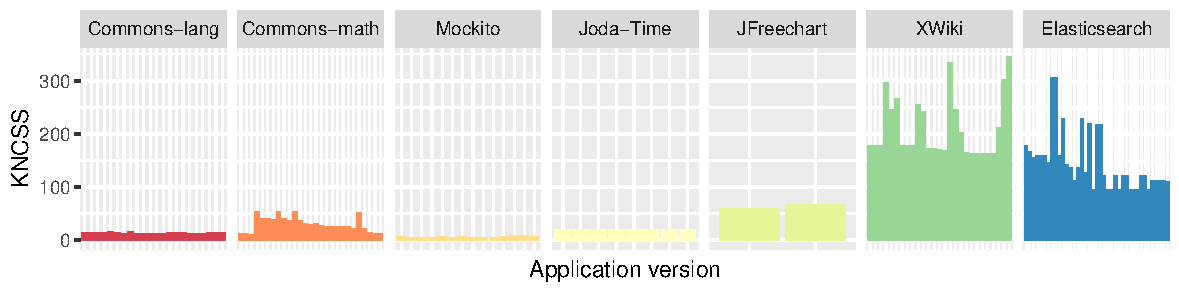
\includegraphics[width=0.98\textwidth]{papers/jcrashpack/benchmark-ncss-per-app-histogram}
    \label{fig:ncssperapp}
  }
  \caption{Complexity and size of the different projects}
  \label{fig:ccnncssperapp}
\end{figure}

Figure \ref{fig:ccnncssperapp} presents the average Cyclomatic Complexity Number (CCN) per method for each project and the Non-Com\-men\-ting Sources Statements (NCSS) per project, ordered by version number, to give an idea of the complexity of a project. Also, Table \ref{tab:benchmark:complexity} gives the number of versions and the average number of non-commenting source statement for each project in \crashpack.
As illustrated in the table and figure, \crashpack contains projects of diverse complexities (the CCN for the least complex project is 1.77, and for the most complex is 3.38) and sizes (the largest project has 177,840 statements, and the smallest one holds 6,060 statements on average), distributed among different versions.

\begin{table*}[t]
	\centering
	\caption{The number of versions and average number of statements ($\overline{NCSS}$) for each project.}
	\label{tab:benchmark:complexity}
	\begin{tabular}{ l | c r } \textbf{Applications} & \textbf{Number of versions} & \textbf{$\overline{NCSS}$}\\
\hline 
\textbf{ Commons-lang } & 22 & 13.38k \\
\textbf{ Commons-math }  & 27 & 29.98k \\
\textbf{ Mockito } & 14 & 6.06k \\
\textbf{ Joda-Time } & 8 & 19.41k \\
\textbf{ JFreechart } & 2 & 63.01k \\
\textbf{ XWiki } & 32 & 177.84k \\
\textbf{ Elasticsearch } & 46 & 124.36k \\
\textbf{ Total } & 151 & 62.01k \\
\end{tabular}
\end{table*}

\begin{table*}[t]
	\centering
	\caption{Number of stack traces (\textit{st}), total number of frames (\textit{fr}), and average number of frames ($\overline{fr}$) and standard deviation ($\sigma$) per stack trace for the different exceptions: NullPointerException (NPE), IllegalArgumentException (IAE), ArrayIndexOutOfBoundsException (AIOOBE), ClassCastException (CCE), StringIndexOutOfBoundsException (SIOOBE), IllegalStateException (ISE), and other exceptions types (Other). }
	\label{tab:benchmark}
%	\input{benchmark-exceptionsapps-table.tex}
    \begin{scriptsize}
	% NullPointerException (NPE), IllegalArgumentException (IAE), ArrayIndexOutOfBoundsException (AIOOBE), ClassCastException (CCE), StringIndexOutOfBoundsException (SIOOBE), IllegalStateException (ISE), Other (Other), 
\begin{tabular}{ l l | r r r r r r r | r } \textbf{Applications} & & \textbf{\rotatebox{90}{ NPE }} & \textbf{\rotatebox{90}{ IAE }} & \textbf{\rotatebox{90}{ AIOOBE }} & \textbf{\rotatebox{90}{ CCE }} & \textbf{\rotatebox{90}{ SIOOBE }} & \textbf{\rotatebox{90}{ ISE }} & \textbf{\rotatebox{90}{ Other }} & \textbf{ Total } \\ 
\hline 
\textbf{ Commons-lang } & \textit{st}  & 5.0 & 3.0 & 2.0 & 0.0  & 6.0 & 0.0  & 6.0 & 22.0\\ 
  & \textit{fr}  & 8.0 & 3.0 & 12.0 & 0.0 & 10.0 & 0.0 & 12.0 & 45.0\\ 
  & $\overline{fr}$  & 1.6 & 1.0 & 6.0 &   & 1.7 &   & 2.0 & 2.0\\ 
 & $\sigma$  & 0.9 & 0.0 & 5.7 &   & 1.0 &   & 1.5 & 2.1\\ 
\hline 
\textbf{ Commons-math } & \textit{st}  & 3.0 & 3.0 & 4.0 & 2.0 & 1.0 & 0.0  & 14.0 & 27.0\\ 
  & \textit{fr}  & 8.0 & 7.0 & 9.0 & 11.0 & 1.0 & 0.0 & 70.0 & 106.0\\ 
  & $\overline{fr}$  & 2.7 & 2.3 & 2.2 & 5.5 & 1.0 &   & 5.0 & 3.9\\ 
 & $\sigma$  & 0.6 & 1.5 & 2.5 & 6.4 & NA &   & 3.0 & 3.0\\ 
\hline 
\textbf{ Mockito } & \textit{st}  & 2.0 & 0.0  & 2.0 & 2.0 & 0.0  & 0.0  & 8.0 & 14.0\\ 
  & \textit{fr}  & 3.0 & 0.0 & 12.0 & 2.0 & 0.0 & 0.0 & 48.0 & 65.0\\ 
  & $\overline{fr}$  & 1.5 &   & 6.0 & 1.0 &   &   & 6.0 & 4.6\\ 
 & $\sigma$  & 0.7 &   & 7.1 & 0.0 &   &   & 3.8 & 4.1\\ 
\hline 
\textbf{ Joda-Time } & \textit{st}  & 0.0  & 3.0 & 0.0  & 0.0  & 0.0  & 0.0  & 5.0 & 8.0\\ 
  & \textit{fr}  & 0.0 & 5.0 & 0.0 & 0.0 & 0.0 & 0.0 & 26.0 & 31.0\\ 
  & $\overline{fr}$  &   & 1.7 &   &   &   &   & 5.2 & 3.9\\ 
 & $\sigma$  &   & 0.6 &   &   &   &   & 1.5 & 2.2\\ 
\hline 
\textbf{ JFreechart } & \textit{st}  & 1.0 & 1.0 & 0.0  & 0.0  & 0.0  & 0.0  & 0.0  & 2.0\\ 
  & \textit{fr}  & 6.0 & 6.0 & 0.0 & 0.0 & 0.0 & 0.0 & 0.0 & 12.0\\ 
  & $\overline{fr}$  & 6.0 & 6.0 &   &   &   &   &   & 6.0\\ 
 & $\sigma$  & NA & NA &   &   &   &   &   & 0.0\\ 
\hline 
\textbf{ XWiki } & \textit{st}  & 20.0 & 4.0 & 0.0  & 6.0 & 1.0 & 0.0  & 20.0 & 51.0\\ 
  & \textit{fr}  & 535.0 & 39.0 & 0.0 & 131.0 & 8.0 & 0.0 & 687.0 & 1400.0\\ 
  & $\overline{fr}$  & 26.8 & 9.8 &   & 21.8 & 8.0 &   & 34.4 & 27.5\\ 
 & $\sigma$  & 33.3 & 3.7 &   & 22.2 & NA &   & 47.0 & 37.0\\ 
\hline 
\textbf{ Elasticsearch } & \textit{st}  & 18.0 & 10.0 & 6.0 & 0.0  & 1.0 & 7.0 & 34.0 & 76.0\\ 
  & \textit{fr}  & 222.0 & 152.0 & 102.0 & 0.0 & 15.0 & 135.0 & 717.0 & 1343.0\\ 
  & $\overline{fr}$  & 12.3 & 15.2 & 17.0 &   & 15.0 & 19.3 & 21.1 & 17.7\\ 
 & $\sigma$  & 9.8 & 9.2 & 18.0 &   & NA & 11.9 & 13.4 & 12.5\\ 
\hline 
 \textbf{Total}  & \textit{st}  & 49.0 & 24.0 & 14.0 & 10.0 & 9.0 & 7.0 & 87.0 & 200.0\\ 
  & \textit{fr}  & 782.0 & 212.0 & 135.0 & 144.0 & 34.0 & 135.0 & 1560.0 & 3002.0\\ 
  & $\overline{fr}$  & 16.0 & 8.8 & 9.6 & 14.4 & 3.8 & 19.3 & 17.9 & 15.0\\ 
 & $\sigma$  & 23.9 & 8.5 & 13.3 & 19.3 & 4.8 & 11.9 & 26.3 & 22.3\\ 
\end{tabular} 
    \end{scriptsize}
\end{table*}

Table \ref{tab:benchmark} shows the distribution of stack traces per exception type for the six most 
common ones, the \textit{Other} category denoting remaining exception types. According to this table, the included stack traces in \crashpack covers different types of the exceptions. Also, they are varied in the size (number of frames): the smallest stack traces have one frame and the largest, a user-defined exception in \textit{Other}, has 175 frames.

\crashpack is extensible and publicly available on GitHub.\footnote{At \url{https://github.com/STAMP-project/JCrashPack}} We provide guidelines to add new crashes to the benchmark and make a pull request to include them in \crashpack master branch.
%
The detailed numbers for each stack trace and its project are available on the \crashpack website.



\section{Running Experiments With ExRunner}
\label{sec:jcrashpack:ExRunner}

\begin{figure}[t]
\centering
\includegraphics[width=0.85\textwidth]{papers/jcrashpack/crashpack-Scheduler}
\caption{\exrunner overview}
\label{fig:exrunner}
\end{figure}

We combine \crashpack with \exrunner, a tool that can be used for running experiments with a given stack trace-based crash reproduction tool. This tool
\begin{inparaenum}[(i)]
\item facilitates the automatic parallel execution of the crash reproduction instances, 
\item ensures robustness in the presence of failures during the crash reproduction failure, and
\item allows to plug different crash reproduction tools to allow a comparison of their capabilities.
\end{inparaenum}

Figure \ref{fig:exrunner} gives an overview of \exrunner architecture.
The \emph{job generator} takes as input the stack traces to reproduce, the path to the Jar files associated to each stack trace, and the configurations to use for the stack trace reproduction tool under study. 
%
For each stack trace, the job generator analyzes the stack frames and discards those with a target method that does not belong to the target system, based on the package name. 
For instance, frames with a target method belonging to the Java SDK or other external dependencies are discarded from the evaluation.
For each configuration and stack trace, the job generator creates a new job description (i.e., a JSON object with all the information needed to run the tool under study) and adds it to a queue. 

To speed-up the evaluation, \exrunner multithreads the execution of the jobs.
The number of threads is provided by the user in the configuration of \exrunner and depends on the resources available on the machine and required by one job execution.
Each thread picks a job from the waiting queue and executes it. 
\exrunner users may activate an observer that monitors the jobs and takes care of killing (and reporting) those that do not show any sign of activity (by monitoring the job outputs) for a user-defined amount of time.
The outputs of every job are written to separate files, with the generated test case (if any) and the results of the job execution (output results from the tool under study).

For instance, when used with \evocrash, the log files contain data about the target method, progress of the fitness function value during the execution, and branches covered by the execution of the current test case (in order to see if the line where the exception is thrown is reached). 
In addition, the results contain information about the progress of search (best fitness function, best line coverage, and if the target exception is thrown), and number of fitness evaluations performed by \evocrash in an output CSV file. 
If \evocrash succeeds to replicate the crash, the generated test is stored separately.

As mentioned by Fraser et al. \cite{FA13challenges}, any research tool developed to generate test cases may face specific challenges. 
One of these is long (or infinite) execution time of the test during the generation process. 
To manage this problem, \evosuite uses a timeout for each test execution, but sometimes it fails to kill sub-processes spawned during the search \cite{FA13challenges}.
We also experienced \evocrash freezing during our evaluation. 
%
In order to handle this problem, \exrunner creates an observer to check the status of each thread executing an \evocrash instance.
If one \evocrash execution does not respond for $10$ minutes (66\% of the expected execution time), the Python script kills the \evocrash process and all of its spawned threads. 

Another challenge relates to garbage collection: we noticed that, at some point of the execution, one job (i.e., one JVM instance) allocated all the CPU cores for the execution of the garbage collector, preventing other jobs to run normally. 
Moreover, since \evocrash allocates a large amount of heap space to each sub-process responsible to generate a new test case (since the execution of the target application may require a large amount of memory) \cite{FA13challenges}, the garbage collection process could not retrieve enough memory and got stuck, stopping all jobs on the machine.
To prevent this behaviour, we set \emph{-XX:ParallelGCThreads} JVM parameter to 1, enabling only one thread for garbage collection, and limited the number of parallel threads per machine, depending on the maximal amount of allocated memory space. 
We set the number of active threads to 5 for running on virtual machines, and 25 for running on two powerful machines. 
Using the logging mechanism in \evocrash, we are able to see when individual executions ran out of memory.

\exrunner is available together with \crashpack.\footnote{See \url{https://github.com/STAMP-project/ExRunner-bash}.}
It has been used to perform benchmarking for search-based crash reproduction approaches, both \evocrash and \botsing (an open-source search-based crash reproduction framework for assessing the new techniques introduced in this thesis), yet it has been designed to be extensible to other available stack trace reproduction tools using a plugin mechanism. 
Integrating another crash reproduction tool requires the definition of two handlers, called by \exrunner: one to run the tool with the inputs provided by \exrunner (i.e. the stack trace, the target frame, and the classpath of the software under test); and one to parse the output produced by the tool to pick up relevant data (e.g., the final status of the crash reproduction, progress of the tool during the execution, \textit{etc}.). 
Relevant data are stored in a CSV file, readily available for analysis.\footnote{ The \exrunner documentation includes a detailed tutorial describing how to proceed, available at \url{https://github.com/STAMP-project/EvoCrash-JCrashPack-application\#run-other-crash-replication-tools-with-exrunner}.}



\section{Application To \evocrash: Setup}
\label{sec:jcrashpack:evocrashevalsetup}

Having \crashpack available allowed us to perform an extensive evaluation of \evocrash, a state-of-the-art tool in search-based crash replication~\cite{Soltani2018a}.
Naturally, our first research question deals with the capability of \evocrash to reproduce crashes from \crashpack: 
%
\begin{itemize}
    \item[\textbf{RQ$_{1.1}$}] \textit{To what extent can \evocrash reproduce crashes from \crashpack?}
\end{itemize}
%
Since the primary goal of our evaluation is to identify current limitations, we refine the previous research question to examine which frames of the different crashes \evocrash is able to reproduce:
%
\begin{itemize}
    \item[\textbf{RQ$_{1.2}$}] \textit{To what extent can \evocrash reproduce the different frames of the crashes from \crashpack?}
\end{itemize}
%
The diversity of crashes in \crashpack also allows us to investigate how certain types of crashes affect reproducibility.
Thus, we investigate whether the exception type and  the project nature have an influence on the reproduction rate:
\begin{itemize}
   \item[\textbf{RQ$_{2.1}$}] \textit{How does project type influence performance of \evocrash for crash reproduction?}
\end{itemize}
In addition, different types of projects might have impact on how costly it is to reproduce the reported crashes for them.
The second research question studies the influence of the exception and project type on the performance of \evocrash:
%
\begin{itemize}
   \item[\textbf{RQ$_{2.2}$}] \textit{How does exception type influence performance of \evocrash for crash reproduction?}
\end{itemize}
%
Finally, we seek to understand why crashes could \emph{not} be reproduced:
%
\begin{itemize}
    \item[\textbf{RQ$_{3}$\phantom{y}}] \textit{What are the main challenges that impede successful search-based crash reproduction?}
\end{itemize}

\subsection{Evaluation Setup}
\label{se:evalsetup}

\paragraph{Number of executions.}

Due to the randomness of Guided Genetic Algorithm in \evocrash, we executed the tool multiple times on each frame. 
The number of executions has to strike a balance between the threats to external validity (i.e., the number of stack traces considered) and the statistical power (i.e., number of runs) \cite{Fraser2014b, Arcuri2014}. 
In our case, we do not compare \evocrash to other tools (see for instance Soltani \etal \cite{soltani2017, Soltani2018a}), but rather seek to identify challenges for crash reproduction. 
Hence we favor external validity by considering a larger amount of crashes compared to previous studies \cite{Soltani2018a} and ran \evocrash 10 times on each frame. In total, we executed 18,590 \evocrash runs.

\paragraph{Search parameters.}

We used the default parameter values \cite{Arcuri2011a, Fraser2014b} with the following additional configuration options: 
we chose to keep the reflection mechanisms, used to call private methods, deactivated.
The rationale behind this decision is that using reflection can lead to generating invalid objects that break the class invariant \cite{Liskov2000} during the search, which results in test cases helplessly trying to reproduce a given crash \cite{Chen2015}.

After a few trials, we also decided to activate the implementation of functional mocking available from \evosuite \cite{arcuri2017private} in order to minimize possible risks of environmental interactions on crash reproduction.
Functional mocking works as follows: when, in a test case, a statement that requires new specific objects to be created (as parameters of a method call for instance) is inserted, either a plain object is instantiated by invoking its constructor, or (with a defined probability, left to its default value in our case) a mock object is created. This mock object is then refined using \texttt{when}-\texttt{thenReturn} statements, based on the methods called during the execution of the generated test case. Functional mocking is particularly useful in the cases where the required object cannot be successfully initialized (for instance, if it relies on environmental interactions or if the constructor is accessible only through a factory). 

Investigating the impact of those parameters and other parameters (e.g., cross\-over rate, mutation rate, etc. to overcome the challenges as identified in \textbf{RQ$_3$}) is part of our future work. 

\paragraph{Search budget.}

Since our evaluation is executed in parallel on different machines, we choose to express the budget time in terms of number of fitness evaluations: i.e., the number of times the fitness function is called to evaluate a generated test case during the execution of the guided generic algorithm. We set this number to 62,328, which corresponds to the average number of fitness evaluations performed by \evocrash when running it during 15 minutes on each frame of a subset of 4 randomly selected stack traces on one out of our two machines. Both of the machines have the same configuration: A cluster running Linux Ubuntu 14.04.4 LTS with 20 CPU-cores, 384 GB memory, and a 482 GB hard drive.

We partitioned the evaluation into two, one per available machine: all the stack traces with the same kind of exception have been run on one machine for 10 rounds.
%
For each run, we measure the number of fitness evaluations needed to achieve reproduction (or the exhaustion of the budget if \evocrash fails to reproduce the crash) and the best fitness value achieved by \evocrash (0 if the crash is reproduced and higher otherwise).
%
The whole process is managed using \exrunner.
The evaluation itself was executed during 10 days on our 2 machines.

\section{Application To \evocrash: Results}
\label{sec:jcrashpack:evocrashevalresults}

In this section, we answer the first two research questions on the extent to which the selected crashes and their frames were reproduced and the impact of the project and the exception type on the performance of \evocrash.
%
We detail the results by analyzing the outcome of \evocrash  in a majority of 10 executions for each frame of each stack trace. We classify the outcome of each execution in one of the five following categories:
\begin{itemize}
\item[] \textbf{reproduced:} when \evocrash generated a test that successfully reproduced the stack trace at the given frame level; 
\item[]\textbf{ex. thrown:} when \evocrash generated a test that cannot fully reproduce the stack trace, but covers the target line and throws the desired exception. The frames of the exception thrown, however, do not contain all the original frames;
\item[]\textbf{line reached:} when  \evocrash generated a test that covers the target line, but does not throw the desired exception;
\item[]\textbf{line not reached:} when none of the tests produced by \evocrash could cover the target line within the available time budget;
and \item[]\textbf{aborted:} when \evocrash could not generate an initial population to start the search process.
\end{itemize}
%
Each outcome denotes a particular state of the search process. For the \emph{reproduced} frames, \evocrash could generate a crash-reproducing test within the given time budget (here, 62,328 fitness evaluations). For the frames that could not be reproduced, either \evocrash exhausted the time budget (for \emph{ex. thrown}, \emph{line reached}, and \emph{line not reached} outcomes) or could not perform the guided initialization (i.e., generate at least one test case with the target method) and did not start the search process (\emph{aborted} outcomes). 
For instance, if the class in the target frame is abstract, \evocrash may fail to find an adequate implementation of the abstract class to instantiate an object of this class during the guided initialization.

\subsection{Crash Reproduction Outcomes (RQ1)}

For \textbf{RQ$_1$},  we first look at the reproduced and non-reproduced crashes to answer \textbf{RQ$_{1.1}$}. 
If \evocrash was successful in reproducing any frame of a stack trace in a majority of 10 executions, we count the crash as a \textbf{reproduced crash}. Otherwise, we count the crash as \textbf{not reproduced}.
%
To answer \textbf{RQ$_{1.2}$}, we detail the results by analyzing the outcome of \evocrash  in a majority of 10 executions for each frame of each stack trace. 

\begin{figure}[t]
	\centering
%	\includegraphics[width=0.90\textwidth]{rq1_compact.pdf}
	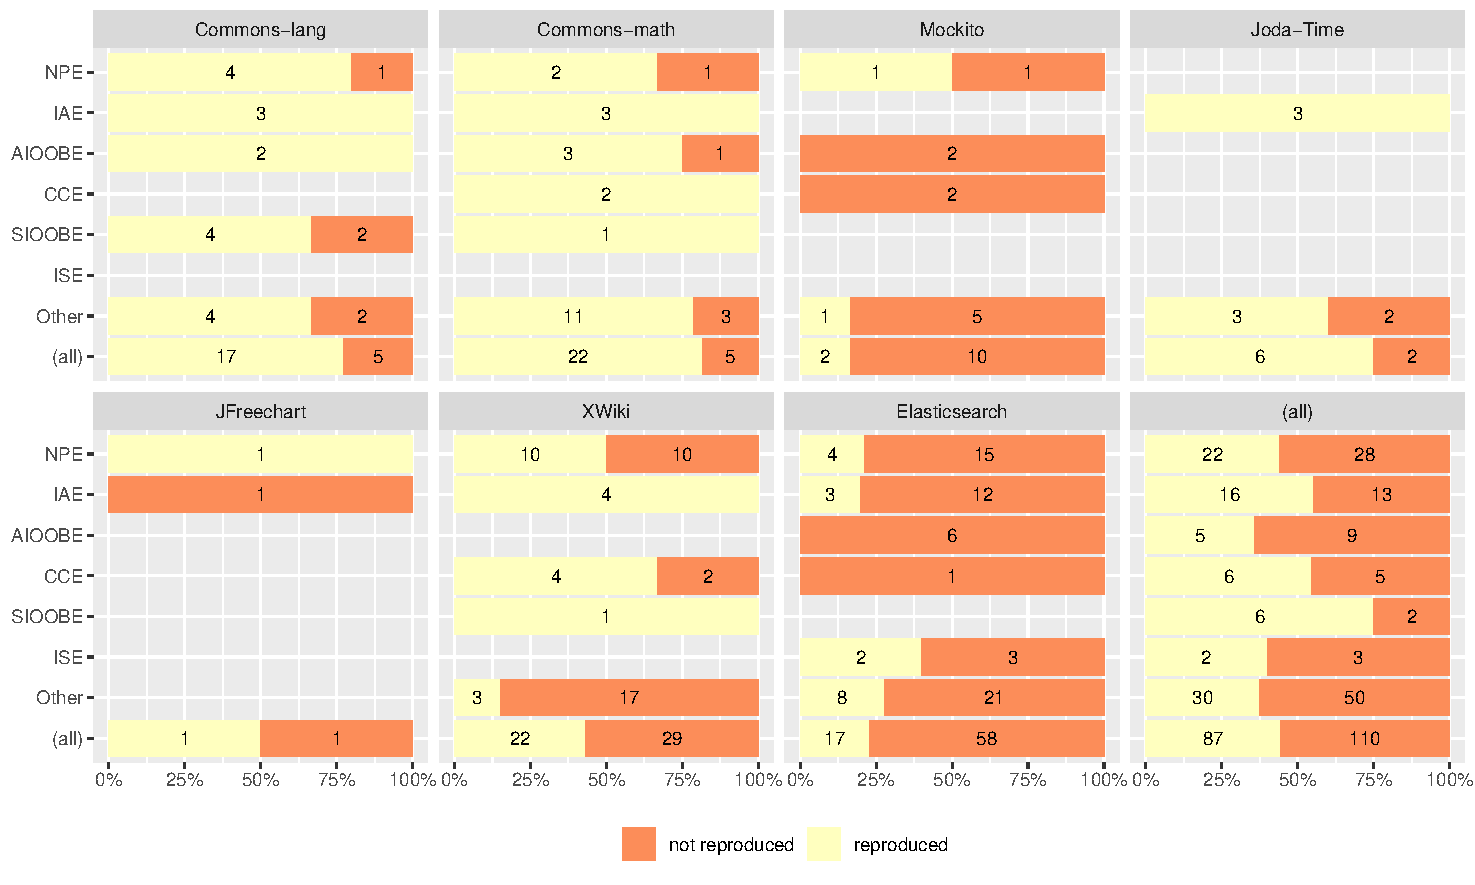
\includegraphics[width=\textwidth]{papers/jcrashpack/rq1_crashes.pdf}
	\caption{Reproduction outcome for the different crashes}
	\label{fig:rq1crashes}
\end{figure}

Figure \ref{fig:rq1crashes} shows the number of reproduced and not reproduced crashes for each project (and all the projects) and type of exception.
\evocrash is successful in reproducing the majority of crashes (more than 75\%) from \textit{Commons-lang}, \textit{Commons-math}, and \textit{Joda-Time}. 
For the other projects, \evocrash reproduced 50\% or less of the crashes, with only 2 out of 12 crashes reproduced for \textit{Mockito}.
%
Crashes with an \textit{IllegalArgumentException} are the most frequently reproduced crashed: 16 out of 29 (55\%).

\begin{figure*}[t]
	\centering
	\subfloat[In each type of exception]{
	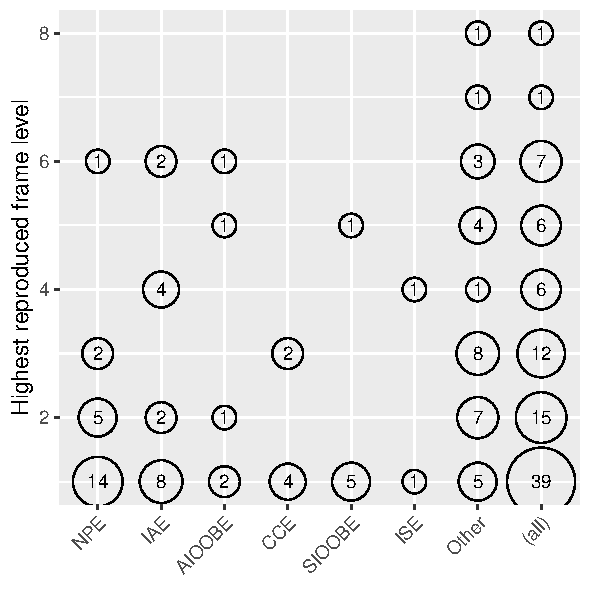
\includegraphics[width=0.48\textwidth]{papers/jcrashpack/rq1_framelvlex.pdf}
	\label{fig:rq1_framelvlex}
	}
	%
	\subfloat[In each type of application]{
	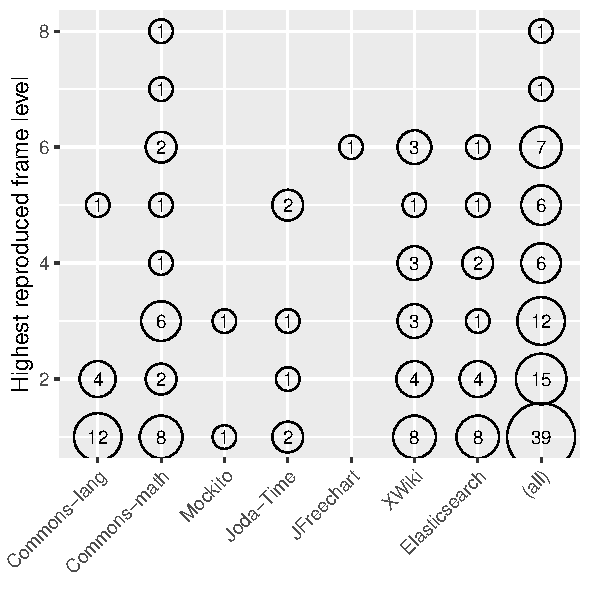
\includegraphics[width=0.48\textwidth]{papers/jcrashpack/rq1_framelvlapp.pdf}
	\label{fig:rq1_framelvlapp}
	}
	\caption{Highest reproduced frame levels}
	\label{fig:highestframe}
\end{figure*}

Before detailing the results of each frame of each crash, we first look at the frame levels that could be reproduced. Figure \ref{fig:highestframe} presents for the 87 stack traces that could be reproduced, the distribution of the highest frame level that could be reproduced for the different crashes for each type of exception (in Figure \ref{fig:rq1_framelvlex}) and each application (in Figure \ref{fig:rq1_framelvlapp}).
As we can see, \evocrash replicates lower frame levels more often than higher levels. 
For instance, for 39 out of  the 87 reproduced stack traces, \evocrash could not reproduce frames beyond level 1 and could reproduce frames up to level 5 for only 9 crashes. 

Figure \ref{fig:rq1_framelvlex} indicates that \evocrash can replicate only the first frame in 14 out of 22 NPE crashes, while there is only one NPE crash for which \evocrash could reproduce a frame above level 3. 
In contrast, it is more frequent for \evocrash to reproduce higher frame levels of IAE stack traces: the highest reproduced frames in 6 out of 16 IAE crashes are higher than 3.
%
Those results suggest that, when trying to reproduce a crash, propagating an illegal argument value trough a chain of method calls (i.e., the frames of the stack trace) is easier than propagating a \texttt{null} value. 
%
According to Figure \ref{fig:rq1_framelvlapp}, \evocrash can reproduce frames higher than 6 only for \textit{Commons-math} crashes. The highest reproduced frames in most of the reproduced crashes in this project are higher than level 2 (12 out of 22). 
In contrast, for \textit{Elasticsearch} the highest reproduced frame is 1 in most of the crashes.

Both the number of crashes reproduced and the highest level at which crashes could be reproduced confirm the relevance of our choice to consider crashes from XWiki and Elasticsearch, for which the average number of frames (resp. 27.5 and 17.7) is higher than for Defects4J projects (at most 6.0 for JFreeChart), as they represent an opportunity to evaluate and understand current limitations. 

\subsubsection{Frames reproduction outcomes} 

\begin{figure}[t]
	\centering
%	\includegraphics[width=0.90\textwidth]{rq1_compact.pdf}
	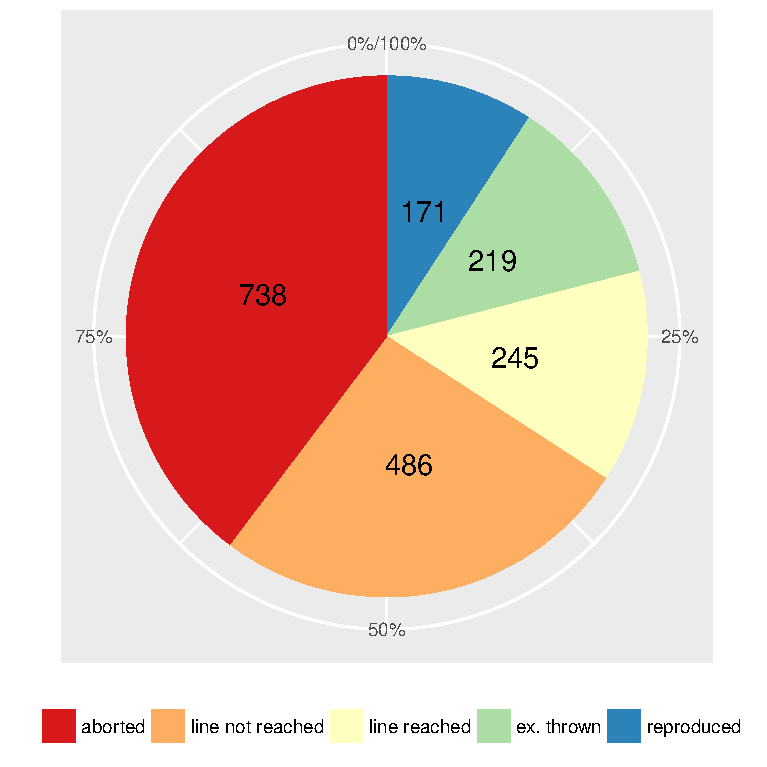
\includegraphics[width=8cm]{papers/jcrashpack/rq1_summary.pdf}
	\caption{An overview of the reproduction outcome}
	\label{fig:rq1summary}
\end{figure}

\begin{figure}[t]
	\centering
%	\includegraphics[width=0.90\textwidth]{rq1_compact.pdf}
	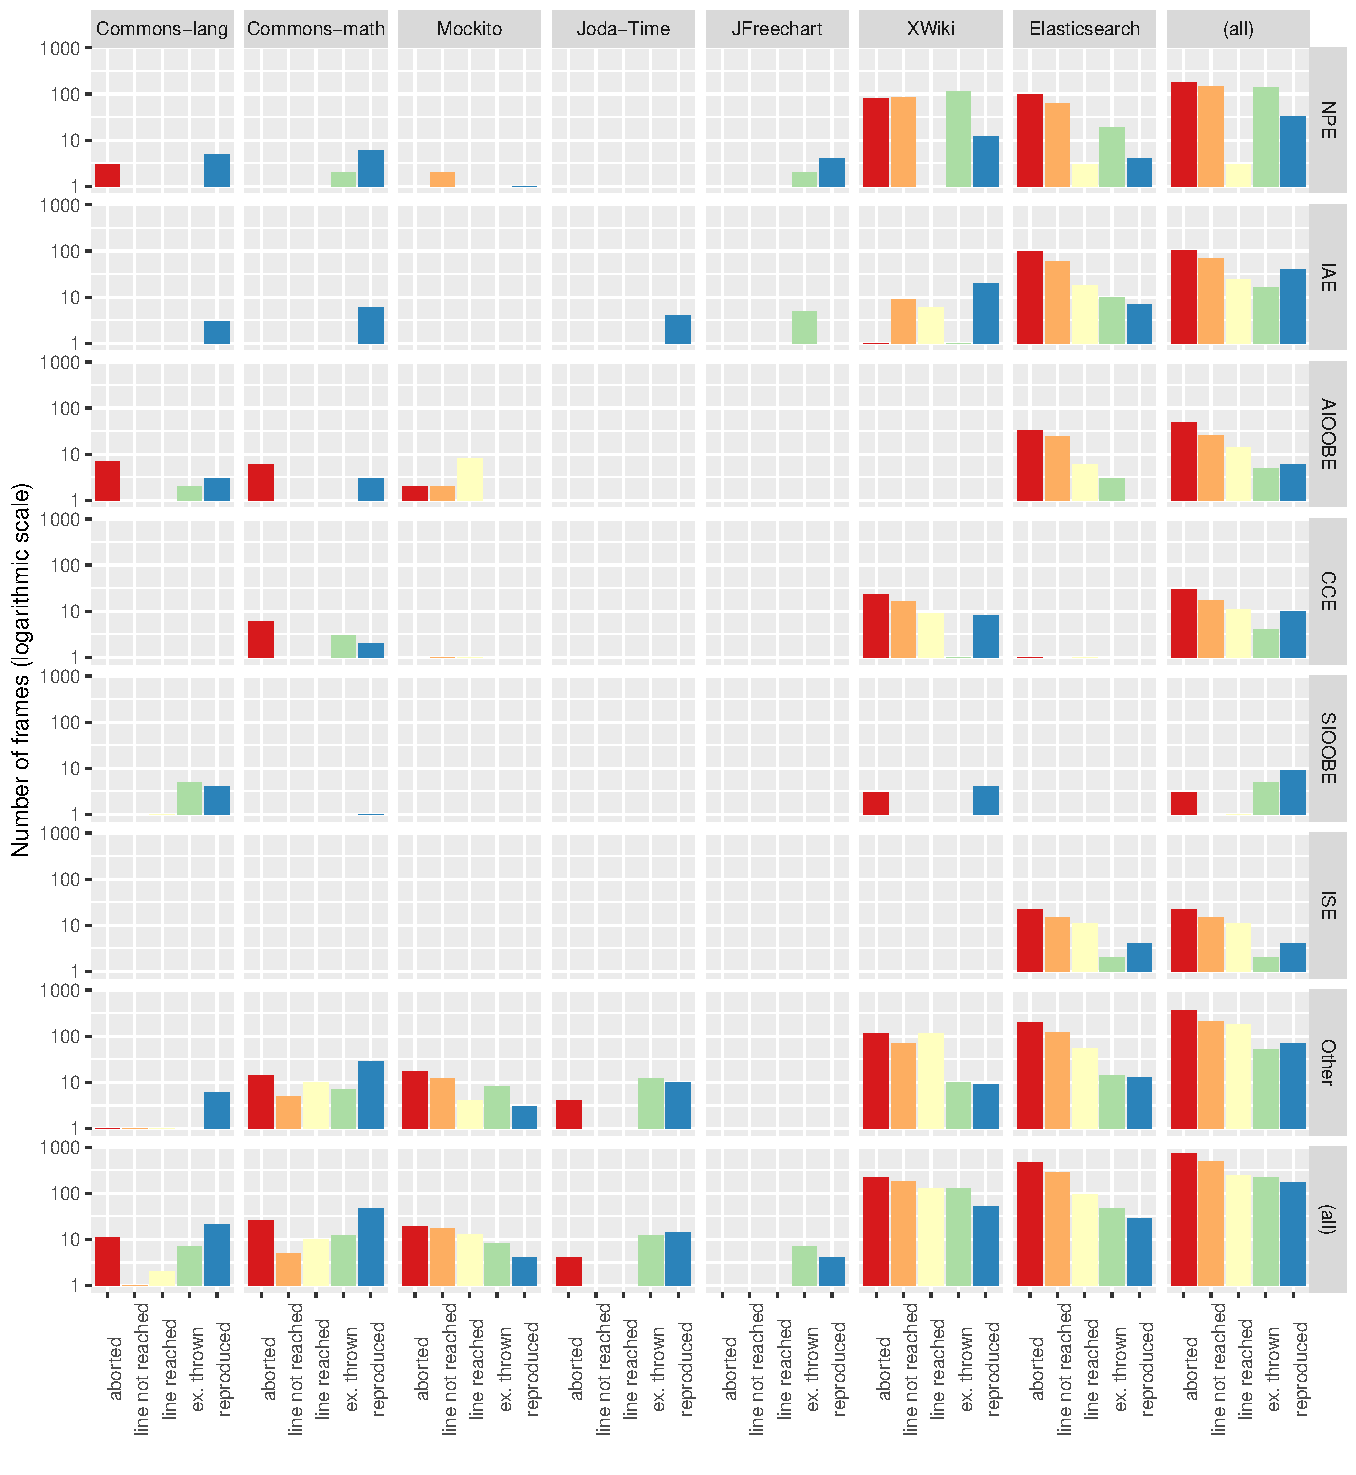
\includegraphics[width=\textwidth]{papers/jcrashpack/rq1_all.pdf}
	\caption{Detailed reproduction outcome for the different frames.}
	\label{figure:outcomecomp}
\end{figure}

To answer \textbf{RQ$_{1.2}$}, we analyze the results for each frame individually.
%
Figure~\ref{fig:rq1summary} presents a summary of the results with the number of frames for the different outcomes. Figure \ref{figure:outcomecomp} details the same results by application and exception. 

Overall, we see in Figure \ref{fig:rq1summary} that \evocrash reproduced 171 frames (out of 1,859), from 87 different crashes (out of 200) in the majority of the ten rounds. If we consider the frames for which \evocrash generated a crash-reproducing test at least once in the ten rounds, the number of reproduced frames increases to 201 (from 96 different crashes).
%
In total, \evocrash exhausted the time budget for 950 frames: 219 with a test case able to throw the target exception, 245 with a test case able to reach the target line, and 486 without a test case able to reach the line. 
\evocrash aborted the search for 738 frames, 455 of which were from Elasticsearch, the application for which \evocrash had the most difficulties to reproduce a stack trace. 

Figure~\ref{figure:outcomecomp} details the results by applications (columns) and exceptions (lines). The last line (resp. column), denoted \textit{(all)}, provides the global results for the applications (resp. exceptions). In the remainder of this section, we discuss the results for the different applications and exceptions. 

\subsubsection{Defects4J applications}

For the Defects4J applications, presented in the first five columns in Figure~\ref{figure:outcomecomp}, in total, 90 (out of 244) of the frames from 48 (out of 71) different crashes were \emph{reproduced}. 
For 94 frames, \evocrash exhausted the time budget (46 \emph{ex. thrown}, 25 \emph{line reached}, and 23 \emph{line not reached}) and \emph{aborted} for 60 frames from the Defects4J projects. 

In particular, only 4 frames out of 61 frames for Mockito were successfully reproduced.
For instance, \evocrash could not reproduce \texttt{MOCKITO-4b}, which has only one frame.
From our evaluation, we observe that one very common problem when trying to reproduce a \textit{ClassCastException} is to find which class should be used to trigger the exception.
%
\begin{lstlisting}[language=Java]
public void noMoreInteractionsWantedInOrder(Invocation undesired){
  throw new VerificationInOrderFailure(join( ...,
		"..." + undesired.getMock() + "':", ...));
}
\end{lstlisting}
%
The exception happens when the \texttt{undesired.getMock()} call returns an object that cannot be cast to \texttt{String}.
During the search, \evocrash mocks the \texttt{undesired} object and assigns some random value to return when the \texttt{getMock} method is called. 
\evocrash generates a test able to cover the target line, but failing to trigger an exception. 
Since the signature of this method is \texttt{Object getMock()}, \evocrash assigns only random \texttt{Object} values to return, where, from the original stack trace, a \texttt{Boolean} value is required to trigger the exception.

\subsubsection{XWiki and Elasticsearch}

XWiki is one of the industrial open source cases in the evaluation, for which 53 (out of 706) frames were successfully \emph{reproduced}, 430 could not be reproduced with the given time budget (125 \emph{ex. thrown}, 127 \emph{line reached}, and 178 \emph{line not reached}), and 223  \emph{aborted} during the generation of the initial population.
%
\evocrash \emph{reproduced} only 28 (out of 909) frames from Elasticsearch, for which, the majority of frames (455) \emph{aborted}  during the generation of the initial population. However, \evocrash was able to start the search for 426 frames (48 \emph{ex. thrown}, 93 \emph{line reached}, and 285 \emph{line not reached}).

\paragraph{Variability of the reproductions.}

We also observed that XWiki and Elasticsearch have the highest variability in their outcomes. 
For XWiki (resp. Elasticsearch), 4 (resp. 3) frames that could be reproduced in a majority of time could however not be reproduced 10 out of 10 times, compared to 2 frames for Commons-lang and Commons-math. 
This could indicate a lack of guidance in the current fitness function of \evocrash. 
For instance, for the Elasticsearch crash ES-26833, \evocrash could only reproduce the third frame 4 times out of 10 and was therefore not considered as reproduced. 
After a manual inspection, we observed that \evocrash gets stuck after reaching the target line and throwing the expected exception. 
From the intermediate test cases generated during the search, we see that the exception is not thrown by the target line, but a few lines after. 
Since the fitness value improved, \evocrash got stuck into a local optima, hence the lower frequency of reproduction  for that frame.\footnote{A detailed analysis is available at \url{https://github.com/STAMP-project/EvoCrash-JCrashPack-application/blob/master/results/manual-analysis/Elasticsearch/ES-26833.md}}
Out future work includes improvement of the guidance in the fitness function and a full investigation of the fitness landscape to decrease the variability of \evocrash outcomes. 


\paragraph{Importance of large industrial applications.}

Compared to Defects4J and XWiki applications, the crash reproduction rate drops from 36.9\% for Defects4J, to 7.5\% for XWiki, and only 3\% for Elasticsearch. Those results emphasize the importance of large industrial applications for the assessment of search-based crash reproduction and enforce the need of context-driven software engineering research to identify relevant challenges \cite{Briand2017a}. 

Additionally to the larger variability of reproduction rate, we observe that frequent use of \textit{Java generics} and \textit{static initialization}, and most commonly, automatically generating suitable input data that resembles \texttt{http} requests are among the major reasons for the encountered challenges for reproducing Elasticsearch crashes.
In Section~\ref{sec:jcrashpack:challenges} we will describe \textbf{14} categories of challenges that we identified as the underlying causes for the presented execution outcomes.

\subsubsection{Exceptions}

The lines in Figure~\ref{figure:outcomecomp} presents the outcomes for the different exceptions. In particular, NPE, IAE, AIOOBE, and CCE are the most represented exceptions in \crashpack. For those exceptions, \evocrash could reproduce, respectively, 32 (out of 499), 40 (out of 250), 6 (out of 99), and 10 (out of 72) frames. Looking at the reproduction frequency, IAE is the most frequently reproduced exception (16\%), followed by CCE (13.8\%), NPE (6.4\%), and AIOOBE (6\%). 

This contrast with the number of frames for which \evocrash aborted the search, where NPE has the lowest frequency (181 frames, 36.2\%), followed by IAE (101 frames, 40.4\%), CCE (30 frames, 41.6\%), and AIOOBE (48 frames, 48.4\%). Interestingly, those numbers show that \evocrash is able to complete the guided initialization for NPEs more often than for other exceptions. 

Figure~\ref{figure:outcomecomp} also shows that the number of test cases that reach the line is low for NPEs, meaning that whenever \evocrash generates at test able to cover the line (\emph{line reached}), the evolution process will be able to progress and generate another test that throws an exception (\emph{ex. thrown}).


\paragraph{\textbf{Summary (RQ$_1$)} To what extent can \evocrash reproduce crashes from \crashpack, and how far it can proceed in the stack traces?}
%
Overall, \evocrash reproduced 171 frames (out of 1,859 - 9\%), from 87 different crashes (out of 200 - 43.5\%) in a majority out of 10 executions. Those numbers climb to 201 frames (10.8\%) from 96 crashes (48\%) if we consider at least one reproduction in one of the 10 executions.
%
In most of the reproduced crashes, \evocrash can only reproduce the first two frames. It indicates that since \evocrash needs higher accuracy in setting the state of the software under test for reproducing higher frames, increasing the length of the stack trace reduces the chance of this tool for crash reproduction. 
%
When looking at larger industrial applications, the crash reproduction rates drop from 36.9\% for Defects4J to 7.5\% for XWiki and 3\% for Elasticsearch.
%
The most frequently reproduced exceptions are IllegalArgumentExceptions. The exceptions for which \evocrash is the most frequently able to complete the guided initialization are NullPointerExceptions.


\subsection{Impact of Exception Type and Project on Performance (RQ2)}

To identify the distribution of fitness evaluations per exception type and project, we filtered the \emph{reproduced} frames out of the 10 rounds of execution.
Tables~\ref{tab:appstats} and~\ref{tab:typestats} present the statistics for these executions, grouped by application and exception types, respectively.

\begin{table*}[t]
\caption{Statistics for the average number of fitness evaluations for the \textit{reproduced} frames (\textbf{fr}) belonging to different stack traces (\textbf{st}), grouped by \textbf{applications}, out of 10 rounds of execution.
The confidence Interval (\textbf{CI}) is calculated for the median bootstrapping with \textit{100,000} runs, at a 95\% confidence level.}
\label{tab:appstats}
\begin{scriptsize}
\begin{tabularx}{0.945\textwidth}{ l r r r r r r r r } 
\hline 
\textbf{Applications} & \textbf{st} & \textbf{fr}& \textbf{Min} & \textbf{Lower Quart.} & \textbf{Median CI} & \textbf{Med.} & \textbf{Upper Quart.} & \textbf{Max} \\ 
\hline 
\textbf{ Com.-lang } & 19  & 213  & 1  & 2.0  & [ 5.0 ,22.0] & 15.0  & 237.0  & 52,240  \\ 
\textbf{ Com.-math } & 24  & 471  & 1  & 13.0  & [ 124.0 ,211.0] & 178.0  & 1,046.5  & 58,731  \\ 
\textbf{ Mockito } & 2  & 40  & 1  & 1.0  & [ 1.0 ,1.0] & 1.0  & 5.2  & 138  \\ 
\textbf{ Joda-Time } & 6  & 138  & 1  & 15.5  & [ 79.1 ,369.0] & 253.5  & 1,290.2  & 40,189  \\ 
\textbf{ JFreechart } & 1  & 41  & 1  & 10.0  & [ -292.0 ,350.0] & 221.0  & 1,188.0  & 20,970  \\ 
\textbf{ XWiki } & 25  & 531  & 1  & 2.5  & [ 14.0 ,30.0] & 23.0  & 209.0  & 34,089  \\ 
\textbf{ Elasticsearch } & 19  & 287  & 1  & 4.0  & [ 5.0 ,32.0] & 23.0  & 125.0  & 17,461  \\ 
\hline 
\textbf{Total} & 96  & 1721  & 1  & 4.0  & [ 34.0 ,59.0] & 48.0  & 534.0  & 58,731  \\ 
\hline 
\end{tabularx} 

\end{scriptsize}
\end{table*}

\begin{table}[t]
\caption{Statistics for the average number of fitness evaluations for the \textit{reproduced} frames (\textbf{fr}) belonging to different stack traces (\textbf{st}), grouped by \textbf{exceptions}, out of 10 rounds of execution.
Confidence Interval (\textbf{CI}) is calculated for median with bootstrapping with \textit{100,000} runs, at 95\% confidence level.}
\label{tab:typestats}
\begin{scriptsize}
\begin{tabularx}{0.94\textwidth}{ l r r r r r r r r} 
\hline 
\textbf{Applications} & \textbf{st} & \textbf{fr}& \textbf{Min} & \textbf{Lower Quart.} & \textbf{Median CI} & \textbf{Med.} & \textbf{Upper Quart.} & \textbf{Max} \\ 
\hline 
\textbf{ NPE } & 26  & 330  & 1  & 6.0  & [ 9.0 ,63.0] & 44.5  & 220.0  & 34,089  \\ 
\textbf{ IAE } & 16  & 399  & 1  & 2.0  & [ 7.0 ,12.0] & 10.0  & 49.0  & 38,907  \\ 
\textbf{ AIOOBE } & 5  & 58  & 1  & 15.5  & [ 252.0 ,1,104.5] & 675.0  & 1,671.2  & 53,644  \\ 
\textbf{ CCE } & 6  & 103  & 1  & 6.5  & [ 74.0 ,210.0] & 120.0  & 560.0  & 10,197  \\ 
\textbf{ SIOOBE } & 8  & 95  & 1  & 12.5  & [ 122.0 ,945.0] & 505.0  & 2,326.0  & 52,240  \\ 
\textbf{ ISE } & 2  & 42  & 1  & 1.0  & [ 1.0 ,3.0] & 2.0  & 105.8  & 1,138  \\ 
\textbf{ Other } & 33  & 694  & 1  & 7.0  & [ 99.0 ,139.0] & 125.5  & 825.0  & 58,731  \\ 
\hline 
\textbf{Total} & 96  & 1721  & 1  & 4.0  & [ 34.0 ,59.0] & 48.0  & 534.0  & 58,731  \\ 
\hline 
\end{tabularx} 

\end{scriptsize}
\end{table}

We filtered out the frames that were not reproduced to analyze the impact of project and exception types on the average number of fitness evaluations and, following recommendations by Arcuri and Briand~\cite{Arcuri2014}, we replaced the test of statistical difference by a confidence interval.
For both groups, we calculated confidence intervals with a  $95\%$ confidence level for medians with bootstrapping with $100,000$ runs.\footnote{We used the \textit{boot} function from the \textit{boot} library in R to compute the \textit{basic} intervals with bootstrapping. See \url{https://github.com/STAMP-project/EvoCrash-JCrashPack-application/tree/master/results} to reproduce the statistical analysis.}

As Table~\ref{tab:appstats} shows, for four projects (Commons-lang, Mockito, XWiki, and Elasticsearch) the median number of fitness evaluations is low.
On the contrary, the cost of crash reproductions for Commons-math, Joda-Time, and JFreechart are  higher in comparison to the rest of projects.
By comparing those results with the projects sizes reported in Table \ref{tab:benchmark:complexity}, where the largest projects are XWiki (with $\overline{NCSS}=177.84k$) and Elasticsearch (with $\overline{NCSS}=124.36k$), we observe that the effort required to reproduce a crash cannot be solely predicted by the project size. 
This is consistent with the intuition that the difficulty of reproducing a crash only depends on the methods involved in the stack trace.

Similarly, according to Figure \ref{fig:ccnperapp}, the average CCN for Mockito, XWiki, and Elasticsearch is lower compared to other projects. 
Table~\ref{tab:appstats} shows that reproducing crashes from these projects is less expensive, and that reproducing crashes from Commons-math, Joda-Time, and JFreechart, which all have higher average CCN, is more expensive.
We also observe that the average CCN for Commons-lang is high, however, contradicting the intuition that crashes from projects higher CCN are more expensive to reproduce, the cost for reproducing crashes in Commons-lang is low compared to other projects.
%
This can be explained by the levels of the frames reproduced by \evocrash: according to Figure \ref{fig:highestframe}, the average level of the reproduced frames in the crashes from Commons-lang is low compared to the other projects and, as we discussed in the previous section, reproducing crashes with fewer frames is easier for \evocrash.

In general, we observe that the performance of \evocrash depends on the complexity of the project and the frame level in the stack trace. Future work includes further investigations to determine which other factors (e.g., code quality) can influence \evocrash performance. 

From Table~\ref{tab:typestats}, we observe that for \textit{CCE}, \textit{SIOOBE}, and \textit{AIOOBE}, the cost of generating a crash-reproducing test case is high, while for \textit{NPE}, \textit{IAE}, and \textit{ISE}, the cost is lower.
One possible explanation could be that generating input data which is in a suitable state for causing cast conflicts, or an array which is in the right state to be accessed by an illegal index is often non-trivial.

In contrast, to trigger an NPE, it is often enough to return a \texttt{null} value not checked by the crashing method.
For example, Listing~\ref{list:NPEexample} shows the stack trace of CHART-4b, a crash from the JFreeChart application.
The crash happens at line \ref{line:NPEcode:crash} of the \texttt{createScatterPlot} method presented in Listing~\ref{list:NPEcode}. 
Listing~\ref{list:NPEtest} shows the test case generated by \evocrash that reproduces the 6th frame (line 6 in Listing~\ref{list:NPEexample}) of the stack trace. 
First, the test initializes the mocks used as mandatory parameters values (from line \ref{line:NPEtest:mock1} to \ref{line:NPEtest:mock2}), before calling the \texttt{createScatterPlot} method (at line \ref{line:NPEtest:crashcall}). The \texttt{ds} \texttt{XYDataset} mock is used along the various calls (from line \ref{line:NPEexample:frame6} to \ref{line:NPEexample:frame1} in Listing~\ref{list:NPEexample}), up to the method \texttt{getDataRange} presented in Listing~\ref{list:XYPlot} that triggers the NPE at line \ref{line:XYPlot:NPE}. In our case, the \texttt{null} value is returned by the \texttt{getRendererForDataset} call with the propagated \texttt{ds} mock at line \ref{line:XYPlot:null}.

\begin{lstlisting}[frame=tb,
  caption={Stack trace for the crash CHART-4b},
  label=list:NPEexample,
  captionpos=t,
  numbers=left,
  firstnumber=0]
java.lang.NullPointerException
	at org.jfree.chart.plot.XYPlot.getDataRange(XYPlot.java:4493)  (*@\label{line:NPEexample:frame1}@*)
	at org.jfree.chart.axis.NumberAxis.autoAdjustRange(NumberAxis.java:434)
	at org.jfree.chart.axis.NumberAxis.configure(NumberAxis.java:417)
	at org.jfree.chart.axis.Axis.setPlot(Axis.java:1044)
	at org.jfree.chart.plot.XYPlot.<init>(XYPlot.java:660)
	at org.jfree.chart.ChartFactory.createScatterPlot(ChartFactory.java:1490) (*@\label{line:NPEexample:frame6}@*)
\end{lstlisting}

\begin{lstlisting}[frame=tb,
  caption={Code excerpt from JFreeChart \texttt{ChartFactory.java}},
  label=list:NPEcode,
  captionpos=t,
  language=Java,
  numbers=left,
  firstnumber=1478]
public static JFreeChart createScatterPlot(String title, String xAxisLabel,
    String yAxisLabel, XYDataset dataset, PlotOrientation orientation,
    boolean legend, boolean tooltips, boolean urls) {

 if (orientation == null) {
  throw new IllegalArgumentException("Null 'orientation' argument.");
 }
 NumberAxis xAxis = new NumberAxis(xAxisLabel);
 xAxis.setAutoRangeIncludesZero(false);
 NumberAxis yAxis = new NumberAxis(yAxisLabel);
 yAxis.setAutoRangeIncludesZero(false);

 XYPlot plot = new XYPlot(dataset, xAxis, yAxis, null);  (*@\label{line:NPEcode:crash}@*)

 [...]
}
\end{lstlisting}

\begin{lstlisting}[frame=tb,
  caption=The test case generated by EvoCrash for reproducing the 6th frame of CHART-4b,
  label=list:NPEtest,
  captionpos=t,
  language=Java,
  numbers=left]
public void test()  throws Throwable  {
 XYDataset ds = mock(XYDataset.class, new ViolatedAssumptionAnswer()); (*@\label{line:NPEtest:mock1}@*)
 doReturn(0).when(ds).getSeriesCount();
 PlotOrientation pl = mock(PlotOrientation.class, new ViolatedAssumptionAnswer()); (*@\label{line:NPEtest:mock2}@*)
 ChartFactory.createScatterPlot((String) null, (String) null, (String) null, ds, pl, true, true, true); (*@\label{line:NPEtest:crashcall}@*)
}
\end{lstlisting}

\begin{lstlisting}[frame=tb,
  caption={Code excerpt from JFreeChart \texttt{XYPlot.java}},
  label=list:XYPlot,
  captionpos=t,
  language=Java,
  numbers=left,
  firstnumber=4490,
  stepnumber=1]
public Range getDataRange(ValueAxis axis) {
 XYItemRenderer r = getRendererForDataset(d); // d == ds and getRendererForDataset(d) returns null (*@\label{line:XYPlot:null}@*)
 [...]
 Collection c = r.getAnnotations(); // r is null and throws a NPE (*@\label{line:XYPlot:NPE}@*)
 [...]
}
\end{lstlisting}

\begin{figure*}[t]
	\centering
	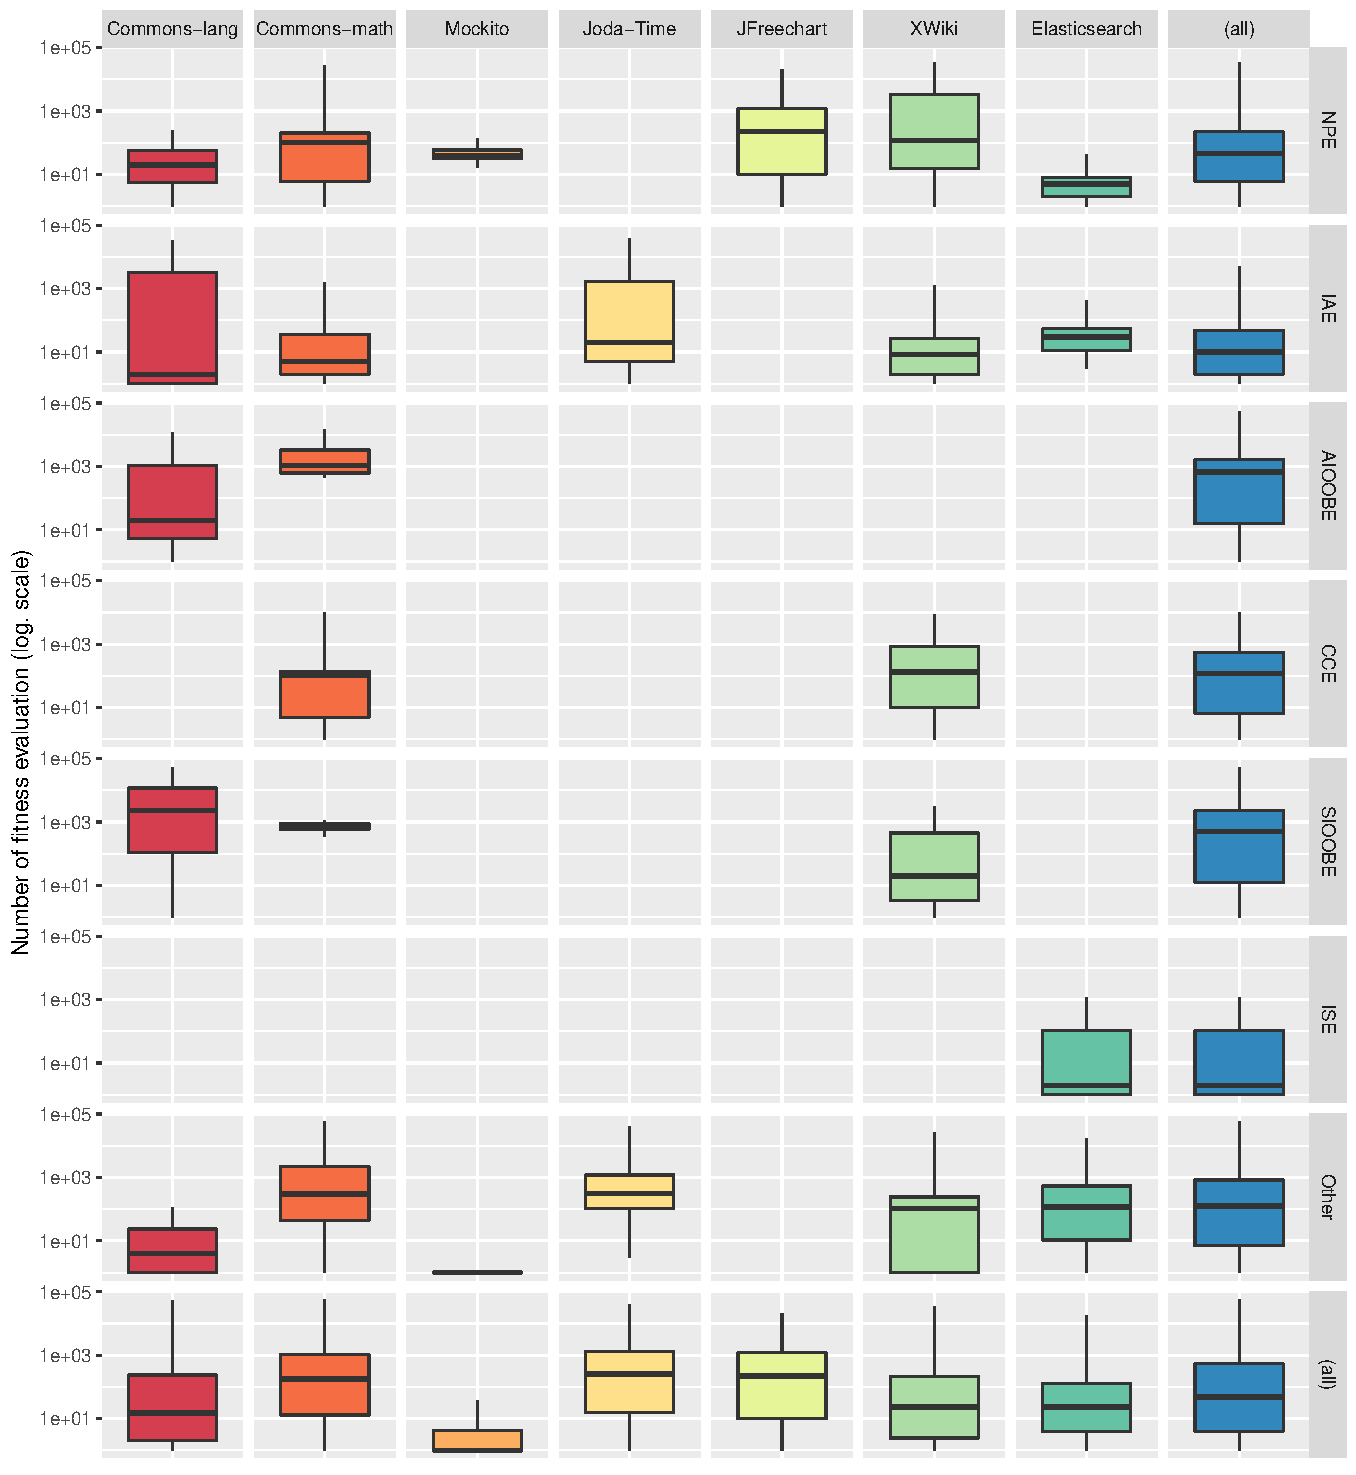
\includegraphics[width=\textwidth]{papers/jcrashpack/rq2_excepappstats.pdf}
	\caption{Average number of fitness evaluations for the \textit{reproduced} frames for each applications and exception type.}
	\label{figure:appexcepstats}
\end{figure*}

Considering the presented results in Figure~\ref{figure:outcomecomp} and Table~\ref{tab:appstats}, crash replication for various exceptions may be dependent on project type.
Figure~\ref{figure:appexcepstats} presents the results of crash reproduction grouped both by applications and exception types.
%
As the figure shows, the cost of reproducing NPE is lower for Elasticsearch, compared to XWiki and JFreechart, and the cost of reproducing IAE is lower for Commons-lang than for Elasticsearch.
We also observe differences in terms of costs of reproducing AIOOBE and SIOOBE for different projects.
%Our results suggest that further investigation in terms of possible correlations between application types and exception types are needed to be able to recommend a adequate number of fitness evaluations to \evocrash users when trying to reproduce a crash for a particular application.


\paragraph{\textbf{Summary (RQ$_{2.1}$)} How does project type influence performance of \evocrash for crash reproduction?}

%To summaries,  the median number of fitness evaluations required to reproduce a crash from Commons-lang, Mockito, XWiki, and Elasticsearch is low, compared to the median number of fitness evaluations needed to reproduce a crash from Commons-math, Joda-Time, and JFreechart. 

We observed that the factors are 
\begin{inparaenum}[(i)]
\item the complexity of the the project, and 
\item the level of the reproduced frames (reproducing higher frame requires more effort).
\end{inparaenum}
Furthermore, we see no link between the size of the project and the effort required to reproduce one of its crashes.


\paragraph{\textbf{Summary (RQ$_{2.2}$)} How does exception type influence performance of \evocrash for crash reproduction?}

For the exceptions, we observe that for ClassCastException, ArrayIndexOutOfBoundsException and StringIndexOutOfBoundsException, the cost of generating a crash-reproducing test case is high, while for NullPointerException, IllegalArgumentException, and IllegalStateException, the cost is lower.
This result indicates that the cost of reproducing types of exceptions for a non-trivial scenario (\textit{e.g.}, class conflicts or accessing an illegal state of an array) needs a more complex input generation. Furthermore, accessing the corresponding complex state is more time consuming for the search process.



\section{Challenges For Crash Reproduction (RQ3)}
\label{sec:jcrashpack:challenges}

\begin{table}[t]
    \centering
	\caption{Challenges with the number and percentage of frames identified for this challenge.}
	\label{tab:challenges}
	\begin{tabular}{l r r} 
\textbf{Category} & \textbf{Frames} & \textbf{Frequency}  
\\\hline 
Input Data Generation & 825 & 49.91\%\\ 
Abstract Class & 242 & 14.64\%\\ 
Anonymous Class & 142 & 8.59\%\\ 
Static Initialization & 141 & 8.53\%\\ 
Complex Code & 118 & 7.14\%\\ 
Private Inner Class & 56 & 3.39\%\\ 
Environmental Dependencies & 52 & 3.15\%\\ 
Irrelevant Frame & 37 & 2.24\%\\ 
Unknown Sources& 16 & 0.97\%\\ 
Nested calls & 10 & 0.60\%\\ 
try/catch & 7 & 0.42\%\\ 
Interface & 6 & 0.36\%\\ 
Empty Enum Type & 1 & 0.06\%\\ 
\hline 
\textbf{Total} & 1653 & 100\% \\ 
\end{tabular}
\end{table}

To identify open problems and future research directions, we manually analyzed the execution logs of 1,653 frames that could not be reproduced in any of the 10 executions.
This analysis includes a description of the reason why a frame could not be reproduced.\footnote{Available at \url{https://github.com/STAMP-project/EvoCrash-JCrashPack-application/tree/master/results/manual-analysis}.}
Based on those descriptions, we grouped the reason of the different failures into 13 categories and identified future research directions.
%This manual process took 9 person-weeks in total.
%
Table \ref{tab:challenges} provides the number and frequency of frames classified in each category.\footnote{For each category, we provide illustrative examples from \url{https://github.com/STAMP-project/EvoCrash-JCrashPack-application/tree/master/results/examples}.} The complete categorization table is available in our replication package.\footnote{The full table is available at \url{https://github.com/STAMP-project/EvoCrash-JCrashPack-application/blob/master/results/manual-analysis/categorisation.csv}.} 

%We divide the categories into two groups. The first group present categories previously identified in related search-based software testing literature. For each category of this group, we discuss how they impede search-based crash reproduction in particular. The second group presents newly identified categories and, for each category, discuss how they impact search-based crash reproduction, but also how they could affect search-based software testing in general. 

For each challenge, we discuss to what extent it is crash-reproduction-specific and its relation to search-based software testing in general. In particular, for challenges previously identified by the related literature in search-based test case generation, we highlight the differences originating from the crash reproduction context.
%\subsection{Challenges previously identified in search-based software testing}

%Seven of the thirteen challenges directly relate to challenges previously identified for search-based testing in general. We confirm their relevance and highlight the differences originating from the crash reproduction context.


\subsection{Input data generation}

Generating complex input objects is a challenge faced by many automated test generation approaches, including search-based software testing and symbolic execution \cite{braione2017tardis}.
Usually, the input space of each input is large and generating proper data enabling the search process to cover its goals is difficult.

As we can see from Table \ref{tab:challenges}, this challenge is substantial in search-based crash reproduction.
Trying to replicate a crash for a target frame requires to set the input arguments of the target method and all the other calls in the sequence properly such that when calling the target method, the crash happens.
Since the input space of a method is usually large, this can be challenging.
\evocrash uses randomly generated \emph{input arguments} and mock objects as inputs for the target method.
As we described in Section~\ref{sec:jcrashpack:evocrashevalresults}, we observe that a widespread problem when reproducing a \textit{ClassCastException} (CCE) is to identify which types to use as input parameters such that a CCE is thrown.
In the case of a CCE, this information can be obtained from the error message of the exception. Our future work includes harvesting additional information, like error messages, to help the search process. 

We also noticed that some stack traces involving Java \emph{generic types} make \evocrash abort the search after failing to inject the target method in every generated test during the guided initialization phase.
Generating \emph{generic type} parameters is also a recognized challenge for automated testing tools for Java \cite{fraser2014automated}.
To handle these parameters, \evocrash, based on \evosuite's implementation \cite{fraser2014automated}, collects candidate types from \texttt{castclass} and \texttt{in\-stance\-of} operators in Java bytecode, and randomly assign them to the type parameter.
Since the candidate types may themselves have generic type parameters, a threshold is used to avoid large recursive calls to generic types.
One possible explanation for the crashes in these cases could be that the threshold is not correctly tuned for the kind of classes involved in the recruited projects.
Thus, the tool fails to set up the target method to inject to the tests.
Based on the results of our evaluation, handling Java generics in \evocrash needs further investigation to identify the root cause(s) of the crashes and devise effective strategies to address them.

\begin{lstlisting}[frame=tb,
  caption={Excerpt of the stack trace for the crash XWIKI-13708},
  label=list:XWIKI13708,
  captionpos=t,
  numbers=left,
  float=t,
  firstnumber=0]
java.lang.NullPointerException: null
  at com.xpn.xwiki.internal.template.TemplateListener.onEvent(TemplateListener.java:79)
  at org.xwiki.observation.internal.DefaultObservationManager.notify(DefaultObservationManager.java:307)
  at org.xwiki.observation.internal.DefaultObservationManager.notify(DefaultObservationManager.java:269)
  [...]
\end{lstlisting}

\begin{lstlisting}[frame=tb,
  caption={Code excerpt from method \texttt{onEvent} in \texttt{TemplateListener.java}},
  label=list:input-generation:example,
  captionpos=t,
  language=Java,
  numbers=left,
  firstnumber=72,
  float=t,
  stepnumber=1]
public void onEvent(Event event, Object source, Object data) {
  XWikiDocument document = (XWikiDocument) source;

  if (document.getXObject(WikiSkinUtils.SKINCLASS_REFERENCE) != null) {
    if (event instanceof AbstractAttachmentEvent) {
      XWikiAttachment attachment = document.getAttachment(((AbstractAttachmentEvent) event).getName());
      String id = this.referenceSerializer.serialize(attachment.getReference()); // target line (*@\label{line:input-generation:target}@*)
      [...]
    }
  }
}
\end{lstlisting}

For instance, \evocrash cannot reproduce the first frame of crash XWIKI-13708\footnote{\url{https://jira.xwiki.org/browse/XWIKI-13708}}, presented in Listing \ref{list:XWIKI13708}. The target method \texttt{onEvent} (detailed in Listing \ref{list:input-generation:example}) has three parameters.
\evocrash could not reach the target line (line \ref{line:input-generation:target} in Listing \ref{list:input-generation:example}) as it failed to generate a fitted value for the second parameter (\texttt{source}). This (\texttt{Object}) parameter should be castable to \texttt{XWikiDocument} and should return values for \texttt{getXObject()} or \texttt{getAttachment()} (using mocking for instance).

\paragraph{Chosen examples:} 
XWIKI-13708, frame 1;
ES-22922, frame 5;
ES-20479, frame 10.\footnote{See \url{https://github.com/STAMP-project/EvoCrash-JCrashPack-application/blob/master/results/examples/InputDataGeneration.md}.}


\subsection{Complex code}

Generating tests for complex methods is hard for any search-based software testing tool \cite{MarkFlag}. In this study, we indicate a method as complex if 
\begin{inparaenum}[(i)]
\item it contains more than 100 lines of code and high cyclomatic complexity; 
\item it holds nested predicates ~\cite{GordonFlag, MarkFlag}; or
\item it has the \textit{flag problem}~\cite{GordonFlag,McMinn2011}, which include (at least one) branch predicate with a binary (boolean) value, making the landscape of the fitness function flat and turning the search into a random search \cite{MarkFlag}.
\end{inparaenum}

As presented in Section~\ref{sec:background:evocrash:guidedalg}, the first component of the fitness function that is used in \evocrash encodes how close the algorithm is to reach the line where the exception is thrown.
Therefore, frames of a given stack trace pointing to methods with a high code complexity\footnote{In some cases for Elasticsearch, the failing methods have nearly 300 lines of source code.} are more costly to reproduce, since reaching the target line is more difficult.  

Handling complex methods in search-based crash reproduction is harder than in general search-based testing. 
The search process in crash reproduction should cover (in most cases) only one specific path in the software under test to achieve the reproduction. 
If there is a complex method on this path, the search process cannot achieve reproduction without covering it. 
Unlike the more general coverage driven search-based testing approach (with line coverage for instance), where the are usually multiple possible executions paths to cover a goal.

\paragraph{Chosen examples:} 
XWIKI-13096, frame 3;
ES-22373, frame 10.\footnote{See \url{https://github.com/STAMP-project/EvoCrash-JCrashPack-application/blob/master/results/examples/ComplexCode.md}.}


\subsection{Environmental dependencies} 

As discussed by Arcuri et al.~\cite{Arcuri2014b}, generating unit tests for classes which interact with the environment leads to
\begin{inparaenum}[(i)]
\item difficulty in covering certain branches which depend on the state of the environment, and
\item generating flaky tests \cite{Luo2014}, which may sometimes pass, and sometimes fail, depending on the state of the environment. 
\end{inparaenum}
%
Despite the numerous advances made by the search-based testing community in handling environmental dependencies \cite{Arcuri2014b, Fraser2014b}, we noticed that having such dependencies in the target class hampers the search process.
%
Since \evocrash builds on top of \evosuite~\cite{fraser2012whole}, which is a search-based \textit{unit} test generation tool, we face the same problem in the crash reproduction problem as well.

\begin{lstlisting}[frame=tb,
float=t,
  caption=Stack trace for the crash XWIKI-12584,
  label=lst:XWIKI12584,
  captionpos=t,
  basicstyle={\scriptsize\ttfamily},
  numbers=left,
  firstnumber=0,
  breaklines=true,
  breakatwhitespace=true,
  tabsize=3,
  ]
java.lang.ClassCastException: [Ljava.lang.Object; cannot be cast to java.lang.String
  at [...].XWikiHibernateStore.searchDocumentReferencesInternal([...]:2457)
  at [...].XWikiHibernateStore.searchDocumentsNamesInternal([...]:2440)
  at [...].XWikiHibernateStore.searchDocumentsNames([...]:2246)
  at [...].XWikiHibernateStore.searchDocumentsNames([...]:2230)
  at [...].XWikiCacheStore.searchDocumentsNames([...]:373)
  at [...].XWiki.searchDocuments([...]:576)
\end{lstlisting}	

For instance, Listing~\ref{lst:XWIKI12584} shows the stack trace of the crash XWIKI-12584.\footnote{Reported at \url{https://jira.xwiki.org/browse/XWIKI-12584} and analyzed at \url{https://github.com/STAMP-project/EvoCrash-JCrashPack-application/blob/master/results/manual-analysis/Xwiki/XWIKI-12584.md}.} 
During the evaluation, \evocrash could not reproduce any of the frames of this stack trace. 
During our manual analysis, we discovered that, for the four first frames, \evocrash was unable to instantiate an object of class \texttt{XWikiHibernateStore},\footnote{See \url{https://github.com/xwiki/xwiki-platform/blob/xwiki-platform-7.2-milestone-2/xwiki-platform-core/xwiki-platform-oldcore/src/main/java/com/xpn/xwiki/store/XWikiHibernateStore.java}} resulting in an abortion of the search.
Since the class \texttt{XWikiHibernateStore} relies on a connection to an environmental dependency (here, a database), generating unit test requires substantial mocking code\footnote{See \url{https://github.com/xwiki/xwiki-platform/blob/xwiki-platform-7.2-milestone-2/xwiki-platform-core/xwiki-platform-oldcore/src/test/java/com/xpn/xwiki/store/XWikiHibernateStoreTest.java}} that is hard to generate for \evocrash. 
As for input data generation, our future work includes harvesting and leveraging additional information from existing tests to identify and use relevant mocking strategies. 

\paragraph{Chosen examples:} 
ES-21061, frame 4;
XWIKI-12584, frame 4.\footnote{See \url{https://github.com/STAMP-project/EvoCrash-JCrashPack-application/blob/master/results/examples/EnvironmentalDependencies.md}.}


\subsection{Static initialization}

In Java, static initializers are invoked only once when the class containing them is loaded.
As explained by Fraser and Arcuri~\cite{Fraser2014b}, these blocks may depend on static fields from other classes on the classpath that have not been initialized yet, and cause exceptions such as \texttt{NullPointerException} to be thrown.
In addition, they may involve environmental dependencies that are restricted by the security manager, which may also lead to unchecked exceptions being generated.

In our crash reproduction benchmark, we see that about 9\% (see Table \ref{tab:challenges}) of the cases cannot be reproduced as they point to classes that have static initializers.
When such frames are used for crash reproduction with \evocrash, the tool currently aborts the search without generating any crash reproducing test.
%
As Fraser and Arcuri~\cite{Fraser2014b} discuss, automatically determining and solving all possible kinds of dependencies in static initializers is a non-trivial task that warrants dedicated research.

\paragraph{Chosen examples:} 
ES-20045, frames 1 and 2.\footnote{See \url{https://github.com/STAMP-project/EvoCrash-JCrashPack-application/blob/master/results/examples/StaticInitialisation.md}.}


\subsection{Abstract classes and methods}
\label{sec:categoryabstractclasses}

In Java, abstract classes cannot be instantiated.
Although generating coverage driven unit tests for abstract classes is possible (one would most likely generate unit tests for concrete classes extending the abstract one or use a parametized test to check that all implementations respect the contract defined by the abstract class), when a class under test is abstract, \evosuite (as the general test generation tool for java) looks for classes on the classpath that extend the abstract class to create object instances of that class. 
In order to cover (e.g., using line coverage) specific parts of the abstract class, \evosuite needs to instantiate the right concrete class allowing to execute the different lines of the abstract class. 

For crash reproduction, as we can see from Table~\ref{tab:challenges}, it is not uncommon to see abstract classes and methods in a stack trace. 
In several cases from Elasticsearch, the majority of the frames from a given stack trace point to an abstract class.
Similarly to coverage-driven unit test generation, \evocrash needs to instantiate the right concrete class: if \evocrash picks the same class that has generated the stack trace in the first place, then it can generate a test for that class that reproduces the stack trace. 
However, if \evocrash picks a different class, it could still generate a test case that satisfies the first two conditions of the fitness function (section~\ref{sec:background:evocrash:guidedalg}). 
In this last case, the stack trace generated by the test would match the frames of the original stack trace, as the class names and line numbers would differ.
The fitness function would yield a value between 0 and 1, but it may never be equal to~0.

\paragraph{Chosen examples:} 
ES-22119, frames 3 and 4;
XRENDERING-422, frame 6.\footnote{See \url{https://github.com/STAMP-project/EvoCrash-JCrashPack-application/blob/master/results/examples/AbstractClass.md}.}


\subsection{Anonymous classes}

As discussed in the study by Fraser \etal~\cite{fraser2012whole}, generating automated tests for covering anonymous classes is more laborious because they are not directly accessible. 
We observed the same challenge during the manual analysis of crash reproduction results generated by \evocrash.
When the target frame from a given crash stack trace points to an anonymous object or a lambda expression, guided initialization in \evocrash fails, and \evocrash aborts the search without generating any test.

\paragraph{Chosen examples:} 
ES-21457, frame 8;
XWIKI-12855, frames 30 and 31.\footnote{See \url{https://github.com/STAMP-project/EvoCrash-JCrashPack-application/blob/master/results/examples/AnonymousClass.md}.}


\subsection{Private inner classes}

Since it is not possible to access a private inner class, and therefore, not possible to directly instantiate it, it is difficult for any test generation tool in Java to create an object of this class.
As for anonymous classes, this challenge is also present for crash reproduction approaches.
In some crashes, the target frame points to a failing method inside a private inner class.
Therefore, it is not possible to directly inject the failing method from this class during the guided initialization phase, and \evocrash aborts the search.

\paragraph{Chosen example:} 
MATH-58b, frame 3.\footnote{See \url{https://github.com/STAMP-project/EvoCrash-JCrashPack-application/blob/master/results/examples/PrivateInnerClass.md}.}


%\subsection{Crash reproduction related challenges}

%We identified six new challenges (out of thirteen). For each one, we also describe how it can affect search-based software testing in general. 


\subsection{Interfaces}

In 6 cases, the target frame points to an interface.
In Java, similar to abstract classes, interfaces may not be directly instantiated.
In these cases also, \evocrash randomly selects the classes on the classpath that implement the interface and, depending on the class picked by \evocrash, the fitness function may  not reach $0.0$ during the search if the class is different from the one used when the input stack trace has been generated.
%
This category is a special case of \emph{Abstract classes and methods} (described in Section \ref{sec:categoryabstractclasses}), however, since the definition of a default behavior for an interface is a feature introduced by Java~8 \cite{jdk8release} that has, to the best of our knowledge, not been previously discussed for search-based testing, we choose to keep it as a separate category. 

\paragraph{Chosen example:}
ES-21457, frame 9.\footnote{See \url{https://github.com/STAMP-project/EvoCrash-JCrashPack-application/blob/master/results/examples/Interface.md}.}


\subsection{Nested private calls}

In multiple cases, the target frame points to a private method. As we mentioned in Section \ref{sec:jcrashpack:evocrashevalsetup}, those private methods are not directly accessible by \evocrash. 
To reach them, \evocrash detects other public or protected methods which invoke the target method directly or indirectly and randomly choose during the search. 
If the chain of method calls, from the public caller to the target method, is too long, the likelihood that \evocrash may fail to pick the right method during the search increases.

In general, calling private methods is challenging for any automated test generation approach.
For instance, Arcuri \etal \cite{arcuri2017private} address this problem by using the Java reflection mechanism to access private methods and private attributes during the search. 
As mentioned in Section \ref{se:evalsetup}, this can generate invalid objects (with respect to their class invariants) and lead to generating test cases helplessly trying to reproduce a given crash \cite{Chen2015}.

\paragraph{Chosen examples:} 
XRENDERING-422, frames 7 to 9.\footnote{See \url{https://github.com/STAMP-project/EvoCrash-JCrashPack-application/blob/master/results/examples/NestedPrivateCalls.md}.}


\subsection{Empty \texttt{enum} type}

In the stack trace of the ES-25849 crash,\footnote{The analysis is available at \url{https://github.com/STAMP-project/EvoCrash-JCrashPack-application/blob/master/results/manual-analysis/Elasticsearch/ES-25849.md}.} 
the 4th frame points to an empty enumeration Java type.\footnote{See \url{https://github.com/jimczi/elasticsearch/blob/0a4b38b60c2752cdc6de819f5bf3414bd01f88c5/core/src/main/java/org/elasticsearch/index/fielddata/ordinals/GlobalOrdinalsBuilder.java}.} 
Since there are no values in the enumeration, \evocrash was not able to instantiate a value and \emph{aborted} during the initialization of the population.
Frames pointing to code in an empty enumeration Java type should not be selected as target frames and could be filtered out using a preliminary static analysis.

\paragraph{Chosen example:} 
ES-25849, frame 4.

\subsection{Frames with \texttt{try}/\texttt{catch}}

Some frames have a line number that designates a call inside a \texttt{try/catch} block.
When the exception is caught, it is no longer thrown at the specific line given in the trace, rather it is typically handled inside the associated \texttt{catch} blocks.
From what we observed, often catch blocks either
\begin{inparaenum}[(i)]
\item re-throw a checked exception, which yield chained stack traces with information that is not exactly as the input stack trace but can still be used for crash reproduction;
 or \item log the caught exception.
\end{inparaenum}
%
Since \evocrash only considers uncaught exceptions that are generated as the result of running the generated test cases during the search, the logged stack traces is presently no use for crash reproduction. Also, even if a stack trace is recorded to an error log, this stack trace is not the manifestation of a crash \textit{per se}. Indeed, once the exception logged, the execution of the program continues normally. 

For instance, for the crash ES-20298,\footnote{Reported at \url{https://github.com/elastic/elasticsearch/issues/20298} and analyzed at \url{https://github.com/STAMP-project/EvoCrash-JCrashPack-application/blob/master/results/manual-analysis/Elasticsearch/ES-20298.md}} \evocrash cannot reproduce the fourth frame of the crash. This frame points to the following method call in a \texttt{try} and \texttt{catch}:
%
\begin{lstlisting}[language=Java]
try {
    processResponse(response);
} catch (Throwable t) {
    onFailure(t);
}
\end{lstlisting}
%
Even if an exception is thrown by the \texttt{processResponse} method, this exception is caught and logged, and the execution of the program continues normally. 

Generally, if an exception is caught in one frame, it cannot be reproduced (as it cannot be observed) from higher level frames. For instance, for ES-20298, all frames above level 4 cannot be reproduced since the exception is catch in frame 4 and not propagated to the higher frames. 
This property of a crash stack trace implies that, for now, depending on where in the trace such frames exist, only a fraction of the input stack traces can actually be used for automated crash reproduction.
Future development of \evocrash can alleviate this limitation by, additionally to the monitoring of uncaught exceptions, read the error log to affecting the propagation of exceptions during execution. 
However, unlike other branching instructions relying on boolean values, for which classical coverage driven unit test generation can use the \emph{branch distance} (see Section \ref{sec:background:evocrash:guidedalg}) to guide the search \cite{McMinn2004}, there is little guidance offered for \texttt{try/catch} instructions since the branching condition is implicit in one or more instructions in the \texttt{try}. 

\paragraph{Chosen example:} 
ES-14457, frame 4.\footnote{See \url{https://github.com/STAMP-project/EvoCrash-JCrashPack-application/blob/master/results/examples/TryCatch.md}.}


\subsection{Missing line number}

\begin{lstlisting}[frame=tb,
  float=t,
  caption=An excerpt of the stack trace from the crash XRENDERING-422  with missing line numbers,
  label=list:missing,
  captionpos=t,
  basicstyle={\scriptsize\ttfamily},
  numbers=left,
  breaklines=true,
  breakatwhitespace=false,
  tabsize=3]
at org.apache.xerces.parsers.XMLParser.parse(Unknown Source)
at org.apache.xerces.parsers.AbstractSAXParser.parse(Unknown Source)
at org.xml.sax.helpers.XMLFilterImpl.parse(XMLFilterImpl.java:357)
\end{lstlisting}

31 frames in \crashpack have frames with a missing line number, as shown in Listing~\ref{list:missing}.
This happens if the Java files have been compiled without any \emph{debug} information (by default, the Java compiler add information about the source files and line numbers, for instance, when printing a stack trace) or if the frame points to a class part of the standard Java library and the program has been run in the Java Runtime Environment (JRE) and not the JDK.

Since \evocrash currently requires a line number to compute the fitness values during the search, those frames have been ignored during our evaluation and do not appear in the results.
Yet, as frames with missing line number appear in \crashpack (and in other stack traces), we decided to mention this trial here as a search-based crash reproduction challenge.
A possible solution, as the future work, is to relax the fitness function so that it can still approximate fitness if line numbers are missing.

\paragraph{Chosen example:} 
XRENDERING-422.\footnote{The stack trace is available at \url{https://github.com/STAMP-project/EvoCrash-JCrashPack-application/blob/master/evaluation/JarFiles/resources/logs/XWIKI/XRENDERING-422/XRENDERING-422.log}}


\subsection{Incorrect line numbers}

In 37 cases, the target frame points to the line in the source code where the target class or method is defined.
This happens when the previous frame points to an anonymous class or a lambda expression.
Such frames practically cannot be used for crash reproduction as the location they point to does not reveal where exactly the target exception occurs.
One possible solution would be to consider the frame as having a missing line number and use the relaxed fitness function to approximate the fitness. 

\paragraph{Chosen examples:} 
MATH-49b, frames 1 and 4.\footnote{See \url{https://github.com/STAMP-project/EvoCrash-JCrashPack-application/blob/master/results/examples/IrrelevantFrames.md}.}


\subsection{Unknown}

We were unable to identify why \evocrash failed to reproduce 16 frames (out of 1,653 frames manually analyzed). 
In these cases, neither the logs nor the source code could help us understand how the exception was propagated. 
%Therefore, factor which leads \evocrash to fail to reproduce the crash could not be clearly identified.


\paragraph{\textbf{Summary (RQ$_3$)} What are the open problems that need to be solved to enhance search-based crash reproduction?}

Based on the manual analysis of the frames that could not be reproduced at least once out of 10 rounds of executions, we identified 13 challenges for search-based crash reproduction.
We confirmed challenges previously identified in other search-based software testing approaches and specified how they affect search-based crash reproduction. And discovered new challenges, more specific to search-based crash reproduction and explained how the can affect other search-based software testing approaches. 

These challenges are related to the difficulty to generate test cases due to complex input data, environmental dependencies, or complex code; abstraction (static initialization, interfaces, abstract, and anonymous classes); encapsulation mechanisms (private inner classes and nested private calls in the given stack trace) of object-oriented languages; or the selection of the target frame in crash reproduction (in \texttt{try}/\texttt{catch} blocks, in empty enumerations, when the location in the source code is unknown, or when the frame has an incorrect line number).


\section{Discussion}
\label{sec:jcrashpack:discussion}

\subsection{Empirical evaluation for crash reproduction}

Conducting empirical evaluation for crash reproduction is challenging. It requires to collect various artifacts from different sources and to analyze the results to determine, in the case of a negative outcome, the cause that prevents the crash reproduction. Some are easy to fix, like missing dependencies that were added to the project linked to the stack trace, and for which we rerun the evaluation on the stack traces. The others are detailed in Section \ref{sec:jcrashpack:challenges}, and serve to identify future research directions. 

One of the most surprising causes is due to a line mismatch in some stack traces.
During the manual analysis of our results, we found out that three frames in two different stack traces, coming from Defects4J projects, target the wrong lines in the source code: the line numbers in the stack traces point to lines in the source code that cannot throw the targeted exception.
Since the stack traces were collected directly from the Defects4J data (which reports failing tests and their outputs), we tried to regenerate them using the provided test suite and found a mismatch between the line numbers of the stack traces indeed.
We reported those two projects to the Defects4J developers:\footnote{See the issue at \url{https://github.com/rjust/defects4j/issues/142}.} a bug in JDK7~\cite{JDK7024096} causes this mismatch.
Since \evocrash relies on line numbers to guide its search, it could not reproduce the crashes.
We recompiled the source code, updated the stack trace accordingly in \crashpack, and rerun the evaluation for those two stack traces.

Thanks to \crashpack and \exrunner, we are now able to ease empirical evaluation for crash reproduction. \exrunner can be extended to other crash reproduction tools\footnote{See how to extend \exrunner at \url{https://github.com/STAMP-project/ExRunner}.} for comparison, or assess the development of new ideas in existing tools. Our future work also includes the prioritization of crashes from \crashpack to allow quick feedback on new ideas in a fast and automated way~\cite{Alshahwan2018}.


\subsection{Usefulness for debugging}


In our evaluation, we focused on the crash-replication capabilities of \evocrash and identified problems affecting those capabilities. 
We considered the generated tests only to classify the outcomes of the \evocrash generation process but did not assess their actual usefulness for debugging. 

Chen \etal \cite{Chen2015} introduced a usefulness criterion for the crash reproduction approaches. 
According to this criterion, a crash reproducing test is useful to the developers if it covers the buggy frame: i.e., if the target frame for which the reproduction is successful is higher than the frame that points to the buggy method.

In our previous work \cite{Soltani2018a}, we conducted a controlled experiment to assess the usefulness of \evocrash for debugging and bug fixing of two crashes (one from Apache Commons Collections and one from Apache Log4j) with 35 master students. Results show that using a crash-replicating test case generated by \evocrash may help to locate and fix the defects faster. Also, this study confirmed the usefulness criterion defined by the Chen \etal \cite{Chen2015} but also found evidence that test cases categorized as not useful can still help developers to fix the bug. 

Since \crashpack also includes two open source industrial and actively maintained applications, it represents an excellent opportunity to confirm the usefulness of \evocrash in an industrial setting. 
The key idea is to centralize the information in the issue tracker by providing a test case able to replicate the crash reported in an issue in the same issue (as an attachment for instance).
This can be automated using, for instance, a GitHub, GitLab or JIRA plugin that executes \evocrash when a new issue contains a stack trace.
To assess the usefulness of \evocrash in an industrial setting, we plan to setup a case study \cite{Wohlin2012} with our industrial partners. 
Hereafter, we outline the main steps of the evaluation protocol using XWiki as subject: 
\begin{inparaenum}[(i)]
\item select four crashes to fix (two from open issues and two from closed issues) for which \evocrash could generate a crash reproducing test for frame 3 or higher;
\item clone the XWiki Git repository in GitHub and open four issues, corresponding to the four crash;
\item remove the fix for the two fixed issues;
\item for each issue, append the test case generated by \evocrash; \label{item:addtestcases}
\item ask (non-XWiki) developers to fix the issues;
and finally, \item repeat the same steps without adding the test cases generated by \evocrash (i.e., omit step \ref{item:addtestcases}).
\end{inparaenum}
%
We would measure the time required to fix the issues (by asking participants to log that time). For the two previously fixed issues, we will compare the fixes provided by the participants with the fixes provided by XWiki developers. And for the two open issues, we will ask feedback from the XWiki developers through a pull request with the different solutions. 

%However, this evaluation is not trivial and requires a significant effort to either control and observe the environment of the developer when asked to perform a debugging task. 
%Or, to analyze and compare the generated crash-reproducing test with the messages in the issue tracker and the code fix in the code version system, with additional threats to the validity linked to the interpretation of the notes in the issue tracker and of the code fix. 

\subsection{Benchmark building}

\crashpack is the first benchmark dedicated to crash reproduction.
We deliberately made a biased selection when choosing Elasticsearch as the most popular, trending, and frequently-forked project from GitHub.
Elasticsearch was among several other highly ranked projects, which addressed other application domains, and thus were interesting to explore.
In the future, further effort should extend \crashpack, possibly by:
\begin{inparaenum}[(i)]
\item using a \textit{random selection} methodology for choosing projects; 
\item involving industrial projects from other application domains;
and \item automatically collecting additional information about the crashes, the stack traces, and the frames to further understand current strengths and limitations of crash reproduction.
\end{inparaenum}

Building \crashpack required substantial manual effort, not just for finding the issues, but also for collecting the right versions of the system itself and its dependencies needed  to reproduce the given crash.
Since we want it to be representative of current crashes, we need to automate this effort as much as possible: for instance, by mining stack traces from issue tracking systems \cite{Nayrolles2016}.

Despite the benefits that the evaluation infrastructure could get from the inclusion of \crashpack bugs in Defects4J, i.e., the isolation of the bugs to ease replicatbility of the evaluations \cite{just2014defects4j}, we designed \crashpack as a standalone instead of extending Defects4J.
The main reason is that not all bugs in Defects4J manifest as crashes (only 73 out of 395 where selected to be part of \crashpack). 
We also believe that the integration of the two benchmarks is not a smooth and easy process.
Defects4J requires isolation of the buggy and fixed versions of the source code, as wel as a test case able to expose the bug \cite{just2014defects4j}. However, not all issues were fixed at the time we collected the crashes in \crashpack.
Also, XWiki and Elasticsearch are much larger applications (124,000 NCSS for Elasticsearch, 177,000 NCSS for XWiki distributed in a hierarchy of several thousands of Maven projects) compared to the API libraries considered in Defects4J (63,000 NCSS for JFreeChart). 
Only building them with their default test suites already raised several issues. 
For those reasons, isolating the bug, the patch, and the non-regression test cases for such kind of large projects is not a trivial task. 









\section{Future Research Directions For Search-Based Crash Reproduction}
\label{sec:jcrashpack:futurework}

From the evaluation and the challenges derived from our manual analysis, we devise the following future research directions. 
While the same challenge can be addressed in different ways, some requiring technical improvements of \evocrash and other raising new research directions, we focus the discussion of this section on the latter. 

\subsection{Context matters}

While search-based crash-reproduction with \evocrash~\cite{soltani2017,Soltani2018a} outperformed other approaches based on \begin{inparaenum}[(i)]
\item backward symbolic execution \cite{Chen2015},
\item test case mutation \cite{Xuan2015},
and \item model-checking \cite{Nayrolles2017},
\end{inparaenum}
our evaluation shows that the extent to which crashes are reproduced varies.
These results indicate the need for taking various types of contexts and properties of software applications into account when devising an approach to a problem.
Thus, we show that indeed, rather than seeking a universal approach to search-based crash reproduction, it is important to find out and address challenges specific to various types of application domains (e.g., RESTful microservices vs. enterprise wiki applications)\cite{Arcuri2017b}.

Furthermore, search-based crash replication boils down to seeking the execution path that will reproduce a given stack trace.
As with other search-based testing approaches, it faces challenges about \emph{input data generation} during the search when the input space is large.
Previous research on \textit{mocking} and \textit{seeding} \cite{arcuri2017private,Rojas2016} address this problem by using functional mocking and extracting objects and constants from the bytecode.

We believe that \emph{taking context into account} should go one step further for crash replication.
With the development of DevOps \cite{Roche2013} and continuous integration and delivery pipelines, there is an increasing amount of available data on the execution of the software.
Those data can be used to guide the search more accurately.
For instance, by seeding the search using values observed in the execution logs and setting up values for \emph{environmental dependencies} (databases, external services, etc.).


\subsection{Stack trace preprocessing and target frame selection}

Various factors may influence the selection of a target frame in a stack trace.
As observed in our evaluation, when not performed cautiously, this selection leads to unsuccessful executions of \evocrash.
For instance, frames targeting code in a \emph{private inner class}, or \emph{irrelevant} source code location (like, as we observed, class header or annotation) should be discarded before performing the selection.

Frames targeting code in \emph{abstract classes} or \emph{interfaces} (only if the target method is defined in the interface, which is possible from Java 8) may be of some use to find the cause of the crash:  for instance, to identify an incorrect subclass implementation \cite{Liskov2000}.
However, as abstract classes and interfaces cannot be directly instantiated, the stack trace generated by \evocrash can never be exactly the same as the given stack trace.
And, as for \emph{input arguments} and \emph{generic type parameters}, \evocrash has no indication on which subclass to pick, making the search difficult.
In this case, considering higher level frames (i.e., frames that are lower in the stack trace) may help to pick the right subclass.

Those reasons motivate the need to develop \emph{stack trace analysis techniques} in order to help the \emph{selection} of a target frame.
This analysis will discard irrelevant and unknown source location frames and provide a visualization to the developer to have a clear view on what are his or her options, for instance by marking stack traces that point to interfaces and abstract classes and recommend him to pick higher level frames.

For a given stack trace, this analysis will also identify frames pointing to a \emph{try/catch} block.
Those stack traces are commonly reported by users to issue tracking systems but cannot (for now) be completely reproduced by \evocrash.
Further investigation on current error handling practices in Java code \cite{Cabral2007,Coelho2017} and how they are reported by users \cite{Maiga2015} will help us to devise efficient approaches to replicate such stack traces.

\subsection{Guided search}

Besides usage of contextual information to enhance the generation of test cases during the search process, we also consider to enhance the guidance itself.
Search based testing algorithms have several parameters (365 in \evocrash), like population size, search budget, probability of applying crossover and mutation, etc. 
As demonstrated by Arcuri and Fraser \cite{Arcuri2011a}, default parameters values work well on average, but may be fare from optimal for specific frames and stack traces. 
A better characterization of the stack traces in \crashpack, trying different \emph{parameters}, as well as improving the \emph{fitness function} itself are part of our future work.
For instance the fitness function could take other elements into account (e.g., compute a similarity for exception messages).
We will also consider multi-objectives search, where, for a given target frame, reproducing each lower  frame becomes an objective of the search.
We plan to reuse our evaluation infrastructure to compare those different approaches and investigate their different fitness landscapes to gain deeper understanding of the search process for crash reproduction. And eventually devise guidelines on \evocrash settings to maximize crash reproduction for a given stack trace and its characteristics.

\subsection{Improving testability}

Finally, as we observed, code complexity was among the major challenges in crash reproduction with \evocrash.
To improve testability, several testability transformation techniques \cite{McMinn2011, LiBytecodeTT, MarkFlag,MarkFlagRemoval, MarkLoopFlag} have been proposed in the literature so far.
Future research may investigate testability transformation techniques and their impact on search-based crash reproduction.


\section{Threats To Validity}
\label{sec:jcrashpack:threats}
% Threats to Validity

Evaluations of crash reproduction approaches, such as the one we conducted for \evocrash, come with threats to internal validity, external validity, and reliability.
The overarching goal of \crashpack is to reduce such threats for all evaluations of any crash reproduction tool, by offering a curated set of crashes to conduct such evaluations.

Concerning \emph{external validity}, we carefully designed \crashpack so that it offers a mix of small and large systems, as well as of different types of exceptions. Furthermore, it includes open source systems directly developed by industry.
%
Nevertheless, any set is incomplete, which is why we keep \crashpack open for extension, as discussed in Section~\ref{sec:jcrashpack:discussion}.  For example, there still remain several other domains, such as gaming or financial applications, for which there is no representative project in the benchmark. 

With respect to \emph{internal validity}, implementation faults can be a source of confounding factors. These can occur in the tools themselves, such as \evocrash or \evosuite, but also in the infrastructure used to actually conduct the experiment. To address the latter, \crashpack comes with \exrunner, which automates the process of scheduling, executing, monitoring, and reporting crash reproduction attempts.

Concerning \emph{reliability}, \crashpack and \exrunner make it easy to repeat experiments, thus making it possible for researchers to independently replicate each others crash reproduction findings.

Besides these threats partially mitigated by \crashpack, our evaluation of \evocrash comes with additional threats to (internal and external) validity. This particularly relates to the randomized nature of genetic algorithms, which we addressed by running the evaluations 10 times, and following the guidelines by Arcuri and Briand \cite{Arcuri2014} for analyzing the results. 
%
Furthermore, such threats concern the risk of bias during the manual analysis, which we mitigated by using cross-checking: the result of each manual analysis has been validated by at least one other person. 
In case of disagreement, we asked for a third opinion.
%
Finally, our evaluation includes only one tool: \evocrash. Previous work showed that \evocrash performs better than other state-of-the-art crash reproduction tools. 
Unfortunately, since to the best of our knowledge, no other tool was publicly available, we were not able to confirm that conclusion on the crashes in \crashpack. 
We believe that \crashpack enhances the current state-of-the-practice in crash reproduction research by offering a publicly available benchmark for which other tool providers can report their results. 




\section{Conclusion}
\label{sec:jcrashpack:conclusion}
Experimental evaluation of crash reproduction research is challenging, due to the computational resources needed by reproduction tools, the difficulty of finding suitable real life crashes, and the intricacies of executing a complex system so that the crash can be reproduced at all.

To remedy this problem, this chapter sets out to create a benchmark of Java crashes, that can be reused for experimental purposes.
To that end we propose \crashpack and \exrunner, a curated benchmark of 200 real life crashes, and a tool to conduct massive experiments on these crashes.
This benchmark is publicly available and can be used to compare existing and new tools against each other, as well as to analyze how proposed improvements to existing reproduction techniques actually constitute an improvement.

We applied the state of the art search-based Java crash reproduction tool, \evocrash, to \crashpack. Our findings include that the state of the art can reproduce 87 crashes out of 200 in a majority of time, that crash reproduction for industry-strength systems is substantially harder, and that \texttt{NullPointerException}s are generally easiest to reproduce. Furthermore, we identified 13 challenges that crash reproduction research needs to address to strengthen uptake in practice, as well a future research directions to address those challenges.

\crashpack  can be extended in various ways: by including more crashes from other types of applications; by automating the collection of information about the crashes and stack traces to further understand current strengths and limitations of crash reproduction; as well as automating the collection of the crashes themselves. Furthermore, since executing crash reproduction tools on 200 crashes may be time taking, \crashpack could be extended to offer prioritization for benchmarks, based on the known theoretical strengths and limitations if the tools. For instance, by ordering crashes based on the cyclomatic complexity of the involved frames to evaluate search-based or symbolic execution-based crash reproduction approaches. 

Finally, our future work for \evocrash itself include improving input data generation by taking information from the execution context and the application (e.g., existing source code and test cases) into account. We also want to deeper our understanding of stack traces in order to be able to recommend target frames to the developers. Finally, we will improve the search process itself by refining the fitness function to improve the guidance through the different frames of the stack trace.

